\documentclass[12pt,a4paper]{article}
\usepackage[utf8]{inputenc}
\usepackage[T1]{fontenc}
\usepackage[italian]{babel}
\usepackage{geometry}
\geometry{margin=2.5cm}
\usepackage{amsmath,amssymb}
\usepackage{booktabs}
\usepackage{graphicx}
\usepackage{float}
\usepackage{xurl}
\usepackage{hyperref}
\hypersetup{colorlinks=true,linkcolor=black,citecolor=black,urlcolor=blue,linktoc=all,bookmarksnumbered=true,pdfstartview={FitH},pdftitle={Inizializzazione Q-learning con modelli linguistici},pdfauthor={Pietro Fazion}}
\setcounter{tocdepth}{2}
\setcounter{secnumdepth}{2}
\setlength{\parskip}{0.6em}
\setlength{\parindent}{0pt}
\sloppy

\title{Modelli linguistici e Q-learning: inizializzare la tabella dei valori nell'ambiente MiniGrid-DoorKey}
\author{Pietro Fazion\\Universit\`a di Verona}
\date{29 settembre 2026}

\begin{document}
\maketitle

\begin{abstract}
L'ambiente MiniGrid-DoorKey assegna la ricompensa solo quando l'agente raggiunge l'obiettivo finale. Il Q-learning classico impiega molti episodi per registrare il primo successo. Questo documento valuta una singola ipotesi. L'ipotesi prevede l'uso di un modello linguistico per stimare il valore ottimo su un gruppo ridotto di stati. Il sistema inserisce questi valori nella tabella Q prima di iniziare l'addestramento.

Nel run sul seed 1337, l'esperimento principale elabora 20 coppie stato-azione relative ai passaggi decisivi. L'agente inizializzato con il modello linguistico, nella valutazione greedy finale su 100 episodi, raggiunge SR=1.00, cioè il 100\%, con una lunghezza media di 13 passi. Il controllo con gli stessi iperparametri raggiunge anch'esso SR=1.00, ma richiede in media 16 passi e converge più tardi. Nel test multi-seed, lo 0\% (SR=0) nella valutazione greedy su 100 episodi riguarda il solo seed non visto 69694. I dati attuali non consentono di stabilire la generalizzazione, ma costituiscono un ottimo punto di partenza; il lavoro multi-seed potrà indagarla ulteriormente. Nell'accuratezza Top-1 tie-aware del solo seed 1337, il modello gpt-oss-120b seleziona l'azione corretta nel 94.1\% dei casi e presenta un errore medio di 0.0122. I file di log conservano i dati alla base dei confronti.
\end{abstract}
\tableofcontents
\newpage

\section{Il problema}\label{sec:problema}
L'algoritmo Q-learning propaga il valore dall'obiettivo agli stati precedenti \cite{sutton2018}. Le definizioni standard di Processo Decisionale di Markov e l'equazione di Bellman restano invariate.

La ricompensa arriva raramente nelle fasi iniziali. La tabella mantiene valori nulli per molto tempo. L'agente non riceve indicazioni per prendere decisioni.

L'esperimento stima il valore $V_{opt}$ con un modello linguistico su pochi stati. Il codice inserisce i valori nella tabella Q iniziale. L'addestramento prosegue con il Q-learning classico. Il processo non genera ricompense aggiuntive. L'obiettivo temporale resta invariato.

I valori iniziali forniscono un riferimento nei punti decisivi. L'effetto di questa modifica viene valutato confrontando l'agente inizializzato con i controlli.

L'esperimento principale valuta il seed 1337. L'addestramento dura 2000 episodi e usa $\alpha=0.04$ e $\gamma=0.95$. La configurazione inizializzata riceve 20 coppie stato-azione. Nella valutazione greedy finale su 100 episodi, l'agente inizializzato ottiene SR=1.00 con 13 passi medi. Il controllo con gli stessi iperparametri ottiene anch'esso SR=1.00, ma 16 passi medi. Il controllo con $\alpha=0.25$ e $\gamma=0.99$ ottiene SR=1.00 e 16 passi medi. Le metriche di accordo con la politica ottima sono rispettivamente 0.576, 0.527 e 0.556; le perdite di valore medie sono 0.0068, 0.0075 e 0.0066. I dati risiedono nella cartella \path{src/output/agents/}.
I file di salvataggio memorizzano i valori in formato JSON.
La Sezione \ref{sec:init} discute i risultati.

\section{Struttura della repository}\label{sec:repo}
Il codice sorgente e i dati risiedono nella repository ufficiale del progetto. L'indirizzo web \`e \url{https://github.com/ttetrao/llm-guided-rl/tree/main}. La cartella \path{src/} contiene i moduli operativi. I programmi si avviano da questa posizione. Il comando \`e \path{python3 -m src.graph.nome_modulo}. Lo schema si applica a tutti i pacchetti. 
Il pacchetto \path{src/graph/} costruisce il grafo del processo decisionale e seleziona gli stati.
Il pacchetto \path{src/llm/} interroga i modelli linguistici.
Il pacchetto \path{src/evaluate/} genera le metriche e i grafici.
Il pacchetto \path{src/agent/} esegue il Q-learning e gestisce i controlli.
Il pacchetto \path{src/env/} contiene gli adattatori per l'ambiente e definisce le fasi.
Il pacchetto \path{src/docs/} raccoglie le istruzioni testuali per i modelli.

Il modulo \path{src/paths.py} gestisce le destinazioni di salvataggio. I dati finiscono sotto \path{src/output/}. La cartella \path{cache} conserva i grafi. La cartella \path{llm} ospita le risposte dei modelli. La cartella \path{agents} raccoglie i dati degli addestramenti. Le cartelle \path{evaluate} contengono i grafici di riepilogo. Il file \path{src/agent/doorkey_qtable_llminit.py} produce i confronti diretti. I documenti di tesi risiedono in \path{thesis/}.

\subsection{I file JSON prodotti dal codice}\label{subsec:filejson}
Ogni modulo scrive un file per esecuzione e non scrive mai a mano. Il nome del file contiene la configurazione: dimensione della mappa, semi, modello e variante dell'agente. I dati permettono di ricostruire la provenienza dei risultati, mentre i grafici usati nel documento devono essere confrontati con il file esatto che li ha prodotti. I file si leggono in tre tappe: prima la mappa, poi gli stati, poi le risposte del modello e i risultati.

Il file \path{mdp_8x8_seed1337.json} nella cartella \path{cache} \`e il grafo completo. Il campo \path{grid_info} registra le dimensioni, le posizioni di chiave, porta e obiettivo, quella di partenza e l'elenco dei muri. La lista \path{nodes} contiene un elemento per stato, con i cinque campi, la fase, l'indicatore di stato terminale, la mappa in caratteri e il valore ottimo \path{v_value} calcolato per iterazione di valore. Ogni nodo elenca le transizioni per azione, con il nodo di arrivo, la ricompensa e il flag di fine episodio. Due indici completano il file: \path{index} collega la tupla di stato al suo identificatore, \path{adj} collega l'identificatore alla lista dei sette successori. Il file \path{frozenlake_mdp_8x8_slippery_seed1337.json} ha la stessa funzione sull'altro ambiente e aggiunge il numero di stati, il numero di azioni, le buche e la descrizione della mappa generata.

Il file \path{doorkey_states_8x8_seed1337.json} nella stessa cartella \`e l'elenco degli stati interrogati. Il campo \path{buckets} raggruppa gli identificatori per etichetta e \path{bucket_counts} ne d\`a la dimensione. Il campo \path{bottleneck_counts} riporta i nodi per ciascuna delle sei categorie, cos\`i il bilancio della selezione \`e leggibile senza rieseguire il codice. Il file conserva anche gli iperparametri del run pilota, le soglie di successo, l'episodio in cui ogni soglia \`e stata raggiunta e il riferimento al grafo di partenza. Quando la selezione copre pi\`u semi, il nome contiene \path{seeds} seguito dagli identificativi separati da trattini e i dati di ciascun seme finiscono sotto \path{per_seed}. Il file \path{frozenlake_qstates_8x8_slippery_seed1337.json} ripete la struttura per FrozenLake.

I file nella cartella \path{llm} contengono le risposte del modello. Sono elenchi piatti, con una riga per ogni coppia stato-azione e sei righe per stato. Ogni riga ripete i campi dello stato, aggiunge l'azione richiesta, il valore vero, il valore stimato e il testo dell'analisi prodotta dal modello. Il campo \path{v_true} \`e il riferimento con cui la valutazione confronta il modello, e \`e calcolato dal grafo e non dal linguaggio. Il campo \path{analysis} conserva il ragionamento scritto e serve a controllare a mano i casi dubbi. Il formato \`e volutamente identico a quello del grafo: \`e il collegamento fra le due tappe. La variante di FrozenLake aggiunge gli indici di riga e colonna e il tipo di casella, e usa quattro azioni invece di sei.

I file nella cartella \path{agents} contengono gli addestramenti. Il nome termina con una variante: \path{llminit} \`e l'agente con la tabella precompilata, \path{vsame} \`e il controllo con gli stessi iperparametri, \path{vstd} \`e il controllo con una seconda configurazione di parametri. Ogni file descrive una variante di agente. Il campo \path{n_init} dice quanti valori sono entrati nella tabella, \path{input_file} dice da quale file di risposte arrivano, \path{hparams} elenca gli iperparametri usati. La sezione \path{optimal} riporta l'accordo con la politica ottima e la perdita di valore media, con i peggiori casi in elenco. La sezione \path{eval} riporta il tasso di successo e la lunghezza media delle partite di valutazione. Il file chiude con quattro serie, una per episodio, che registrano ricompensa, successo, perdita e lunghezza, e con la tabella Q finale. Le curve dei grafici escono da queste serie.

I file di testo affiancano i JSON. Il file \path{log_valutazione.txt} nella cartella \path{evaluate} raccoglie le metriche di una valutazione; i nomi dei grafici nella cartella \path{grafici} permettono di abbinare ciascun grafico al run usato. Il file \path{speedup_summary.csv} riporta anche soglie e tempi di superamento, ma alcune sue righe descrivono esecuzioni precedenti e non coincidono con tutti i JSON correnti; per questo documento i valori interpretati provengono dai riquadri e dai campi dei grafici effettivamente mostrati.

\section{L'ambiente e il valore ottimo}\label{sec:ambiente}
Il progetto adotta l'ambiente \path{MiniGrid-DoorKey-8x8-v0} \cite{minigrid2023}. Le regole sono originali. L'agente raccoglie la chiave. L'agente apre la porta con l'azione \path{toggle}. L'agente raggiunge l'obiettivo fisso sulla mappa. La ricompensa vale 1 solo sul bersaglio. La ricompensa vale 0 in ogni altra cella. Il limite massimo di passi \`e 450.

Lo stato interno del grafo richiede cinque variabili. Le variabili sono la posizione, la direzione dell'agente, il possesso della chiave e lo stato della porta. La posizione dei muri varia per ogni livello. Queste cinque variabili descrivono la mappa in modo univoco per ogni configurazione.

Lo script \path{src/graph/mdp_graph.py} genera il grafo. Il calcolo considera sette azioni per ogni stato. Il processo determina la cella di arrivo e la ricompensa. Il grafo contiene 480 nodi per ogni layout. Il bersaglio si trova sempre nella stessa cella. Il calcolo applica il metodo della value iteration e un fattore di sconto 0.99 per determinare il valore ottimo $V_{opt}$. Questa operazione fornisce il parametro di valutazione per il modello linguistico. Il processo esclude gli stati finali dalle interrogazioni. Il sistema ignora l'azione nulla.

Lo script \path{src/env/view_wrapper.py} traccia il progresso dell'agente. Lo stato \path{find_key} indica la ricerca della chiave. Lo stato \path{open_door} indica il possesso della chiave e la porta chiusa. Lo stato \path{reach_goal} indica il via libera verso l'obiettivo. L'agente deve rispettare questa sequenza. Due posizioni uguali con stati di avanzamento diversi richiedono azioni diverse.

\section{Selezione degli stati}\label{sec:stati}
L'interrogazione completa dei 480 nodi richiede molto tempo. Molte celle di passaggio condividono lo stesso valore. Un parametro definisce il numero massimo di interrogazioni. Il file \path{src/graph/doorkey_states.py} seleziona gli stati utili.

\subsection{Tipologie di nodi decisivi}\label{subsec:bottleneck}
La funzione \path{extract_bottleneck} dal file \path{src/graph/doorkey_states.py} isola i nodi decisivi dal grafo. Il processo non richiede l'esecuzione di partite. I nodi si dividono in sei categorie.
Con collo di bottiglia si intende una posizione in cui la scelta dell'agente impegna una decisione. La definizione \`e strutturale, non statistica. In quasi tutta la mappa il valore dipende solo dalla distanza dagli oggetti, quindi due mosse diverse portano a risultati equivalenti e un errore si corregge tornando indietro. La situazione cambia in tre punti: la cella della chiave, la cella della porta e l'ultimo passo prima dell'obiettivo. Un errore in un nodo qualsiasi si sposta e si annulla. Un errore in questi nodi cambia la fase del gioco, e la fase non si riporta indietro.

Un nodo del grafo non \`e una casella. Lo stato \`e una tupla di cinque campi: due coordinate, direzione, possesso della chiave e stato della porta. Lo stesso oggetto produce quindi pi\`u nodi. Sulla cella della chiave l'agente la possiede per forza, perch\`e il grafo esclude la combinazione senza chiave. I nodi sono 4 direzioni per 2 stati della porta. Sulla cella della porta vale il viceversa: la porta deve essere aperta, altrimenti la casella \`e un muro. I nodi sono 4 direzioni per 2 stati della chiave. Questo spiega perch\`e un solo oggetto dia 8 nodi e non uno.

Il numero di nodi dipende dalla mappa e non dal codice. Ogni lato accessibile della porta e ogni casella adiacente alla chiave o all'obiettivo genera i propri nodi. I muri decidono quante caselle restano libere. Sulla mappa di base l'unione delle sei categorie contiene 32 nodi su 480, circa il 7\%.
\begin{enumerate}
\item \path{on_key} raccoglie gli stati in cui l'agente occupa la cella della chiave. Sono 8, le 4 direzioni per i 2 stati della porta. L'agente possiede la chiave per costruzione, quindi il campo che la registra non varia. La decisione \`e se proseguire o lasciare la chiave: \path{drop} riporta in fase di ricerca e butta via il cammino fatto.
\item \path{on_door} raccoglie gli stati in cui l'agente occupa la cella della porta aperta. Sono 8, le 4 direzioni per i 2 stati della chiave. La porta deve essere aperta, altrimenti la casella \`e un muro. Da qui la strada verso l'obiettivo resta libera e la porta non si richiude da sola.
\item \path{adj_door} raccoglie gli stati in cui l'agente \`e di fronte alla porta chiusa. La condizione \`e doppia: la direzione punta verso la porta e la porta \`e chiusa. Ogni lato accessibile d\`a 2 nodi, uno con la chiave e uno senza. La categoria conta da 3 a 4 nodi secondo la mappa.
\item \path{door_toggle} raccoglie gli stati in cui \path{toggle} apre davvero la porta. \`E l'incrocio dei due elenchi precedenti: l'agente ha la chiave, la porta \`e chiusa e l'azione cambia lo stato. Sono 2 nodi, uno per lato accessibile della porta.
\item \path{key_take} raccoglie gli stati in cui \path{pickup} acquisisce la chiave. Sono i nodi privi di chiave con l'agente su una casella adiacente e rivolto verso quella della chiave. Ogni casella d\`a 2 nodi, uno per stato della porta, e quante caselle restano libere dipende dai muri. La categoria va da 2 a 8 nodi.
\item \path{goal_entry} raccoglie gli stati che offrono la ricompensa. Sono i nodi non terminali da cui \path{forward} entra nell'obiettivo. Ogni casella adiacente all'obiettivo d\`a 4 nodi, una per combinazione di chiave e porta.
\end{enumerate}
Le categorie non sono disgiunte. I nodi in cui due oggetti si incontrano appartengono a due elenchi insieme, e il loro valore non si ottiene sommando i due casi presi separatamente.

Il bucket \texttt{bottleneck} riceve solo questi nodi. Gli altri portano l'etichetta \path{ckpt} con la soglia di successo. Le due famiglie non si confondono nei dati. Il punto non \`e risparmiare interrogazioni. Il punto \`e che sugli altri nodi l'errore si annulla al passo dopo, e su questi si propaga.

\subsection{Campionamento della progressione}\label{subsec:checkpoint}
I nodi decisivi marcano i passaggi obbligati. I nodi di progressione fotografano l'evoluzione dell'agente nel tempo. L'agente visita molte celle inutili all'inizio. L'agente si concentra sul percorso ottimale alla fine. La funzione \path{run_pilot} dal file \path{src/graph/doorkey_states.py} addestra un agente senza aiuti esterni. I parametri sono $\alpha=0.3$ e $\gamma=0.99$. L'esplorazione decade lentamente.

Il programma salva gli stati visitati quando il successo medio tocca soglie specifiche. Le soglie sono 0.3, 0.5, 0.7, 0.8 e 1.0. I salvataggi per i valori bassi includono tutti i percorsi tentati. I salvataggi per i valori alti aggiungono deviazioni casuali. Questo accorgimento impedisce di registrare solo la sequenza perfetta. Il livello di test attiva le soglie agli episodi 93, 115, 137, 150 e 175. Ogni attivazione salva circa 300 nodi.

Alcuni scenari isolati completano il gioco al primo tentativo per puro caso. Tutte le soglie si attivano simultaneamente. Le liste contengono pochissimi nodi. Il codice riporta questi eventi per tracciamento.

La funzione \path{allocate} dal file \path{src/graph/doorkey_states.py} riserva il primo spazio per i nodi decisivi. Il programma divide il resto della capienza tra i nodi di progressione calcolando i resti maggiori.

\section{Interrogazione del modello}\label{sec:prompt}
Il programma calcola il valore per l'azione $Q$ a partire dal valore dello stato $V$. Il testo di istruzione risiede in \path{src/docs/doorkey/it/prompt.txt}. I file \path{src/llm/query_gpt.py} e \path{src/llm/query_gemma.py} gestiscono le chiamate.

Il modello riceve le regole del gioco e la legenda della mappa. Il testo include le definizioni per il calcolo del valore. Il programma invia la mappa corrente e le sei mappe relative alle possibili mosse. Il modello linguistico valuta solo la distanza dall'obiettivo per ogni opzione. L'espressione valutata \`e $\gamma^d$ con $\gamma=0.99$. Il calcolo sfrutta il determinismo del gioco. Il valore esatto di uno stato distante $d$ mosse corrisponde a $\gamma^d$. Il modello non adopera stime casuali. Il modello risponde nel formato JSON. Ogni risposta include l'applicazione della regola, il conteggio dei passi e il calcolo numerico. Il programma scarta le risposte anomale o errate.

Il test principale impiega il modello gpt-oss-120b su un livello di base. I file occupano la cartella \path{src/output/llm/}. Il file di output attualmente presente contiene 870 record, mentre le figure dello scenario base sono state prodotte da una valutazione precedente con 85 stati validi su 99 richieste. Questa differenza di provenienza non cambia le metriche lette nei grafici, ma impedisce di usare il JSON corrente per ricostruirle senza eseguire nuovamente la valutazione. Il codice attende 65 secondi tra una chiamata e l'altra e ritenta fino a 3 volte in caso di errore.

Un secondo test analizza cinque livelli differenti. Il file di output relativo contiene 930 record e 629 stime valide; la valutazione considerata dai grafici usa 111 stati validi.

\section{Precisione dei valori}\label{sec:qualita}
Lo script \path{src/evaluate/evaluate_llm.py} calcola le metriche. I risultati riempiono il file \path{src/output/evaluate/log_valutazione.txt}. L'analisi confronta il valore calcolato dal modello linguistico con il valore reale della mappa.

Nel valutare il modello linguistico bisogna distinguere i valori assoluti dalle scelte Top-k: le due misure descrivono aspetti diversi. Sullo scenario di base l'errore medio assoluto è 0.0122 e il 97.4\% delle risposte ha un errore inferiore a 0.05. I dati aggregati dei cinque layout contengono 155 stati, dei quali 44 risultano falliti (44/155=28.4\%) e 111 validi; per questi dati l'errore medio assoluto è 0.0153 e il 96.8\% delle risposte resta sotto 0.05.

\begin{figure}[H]
\centering
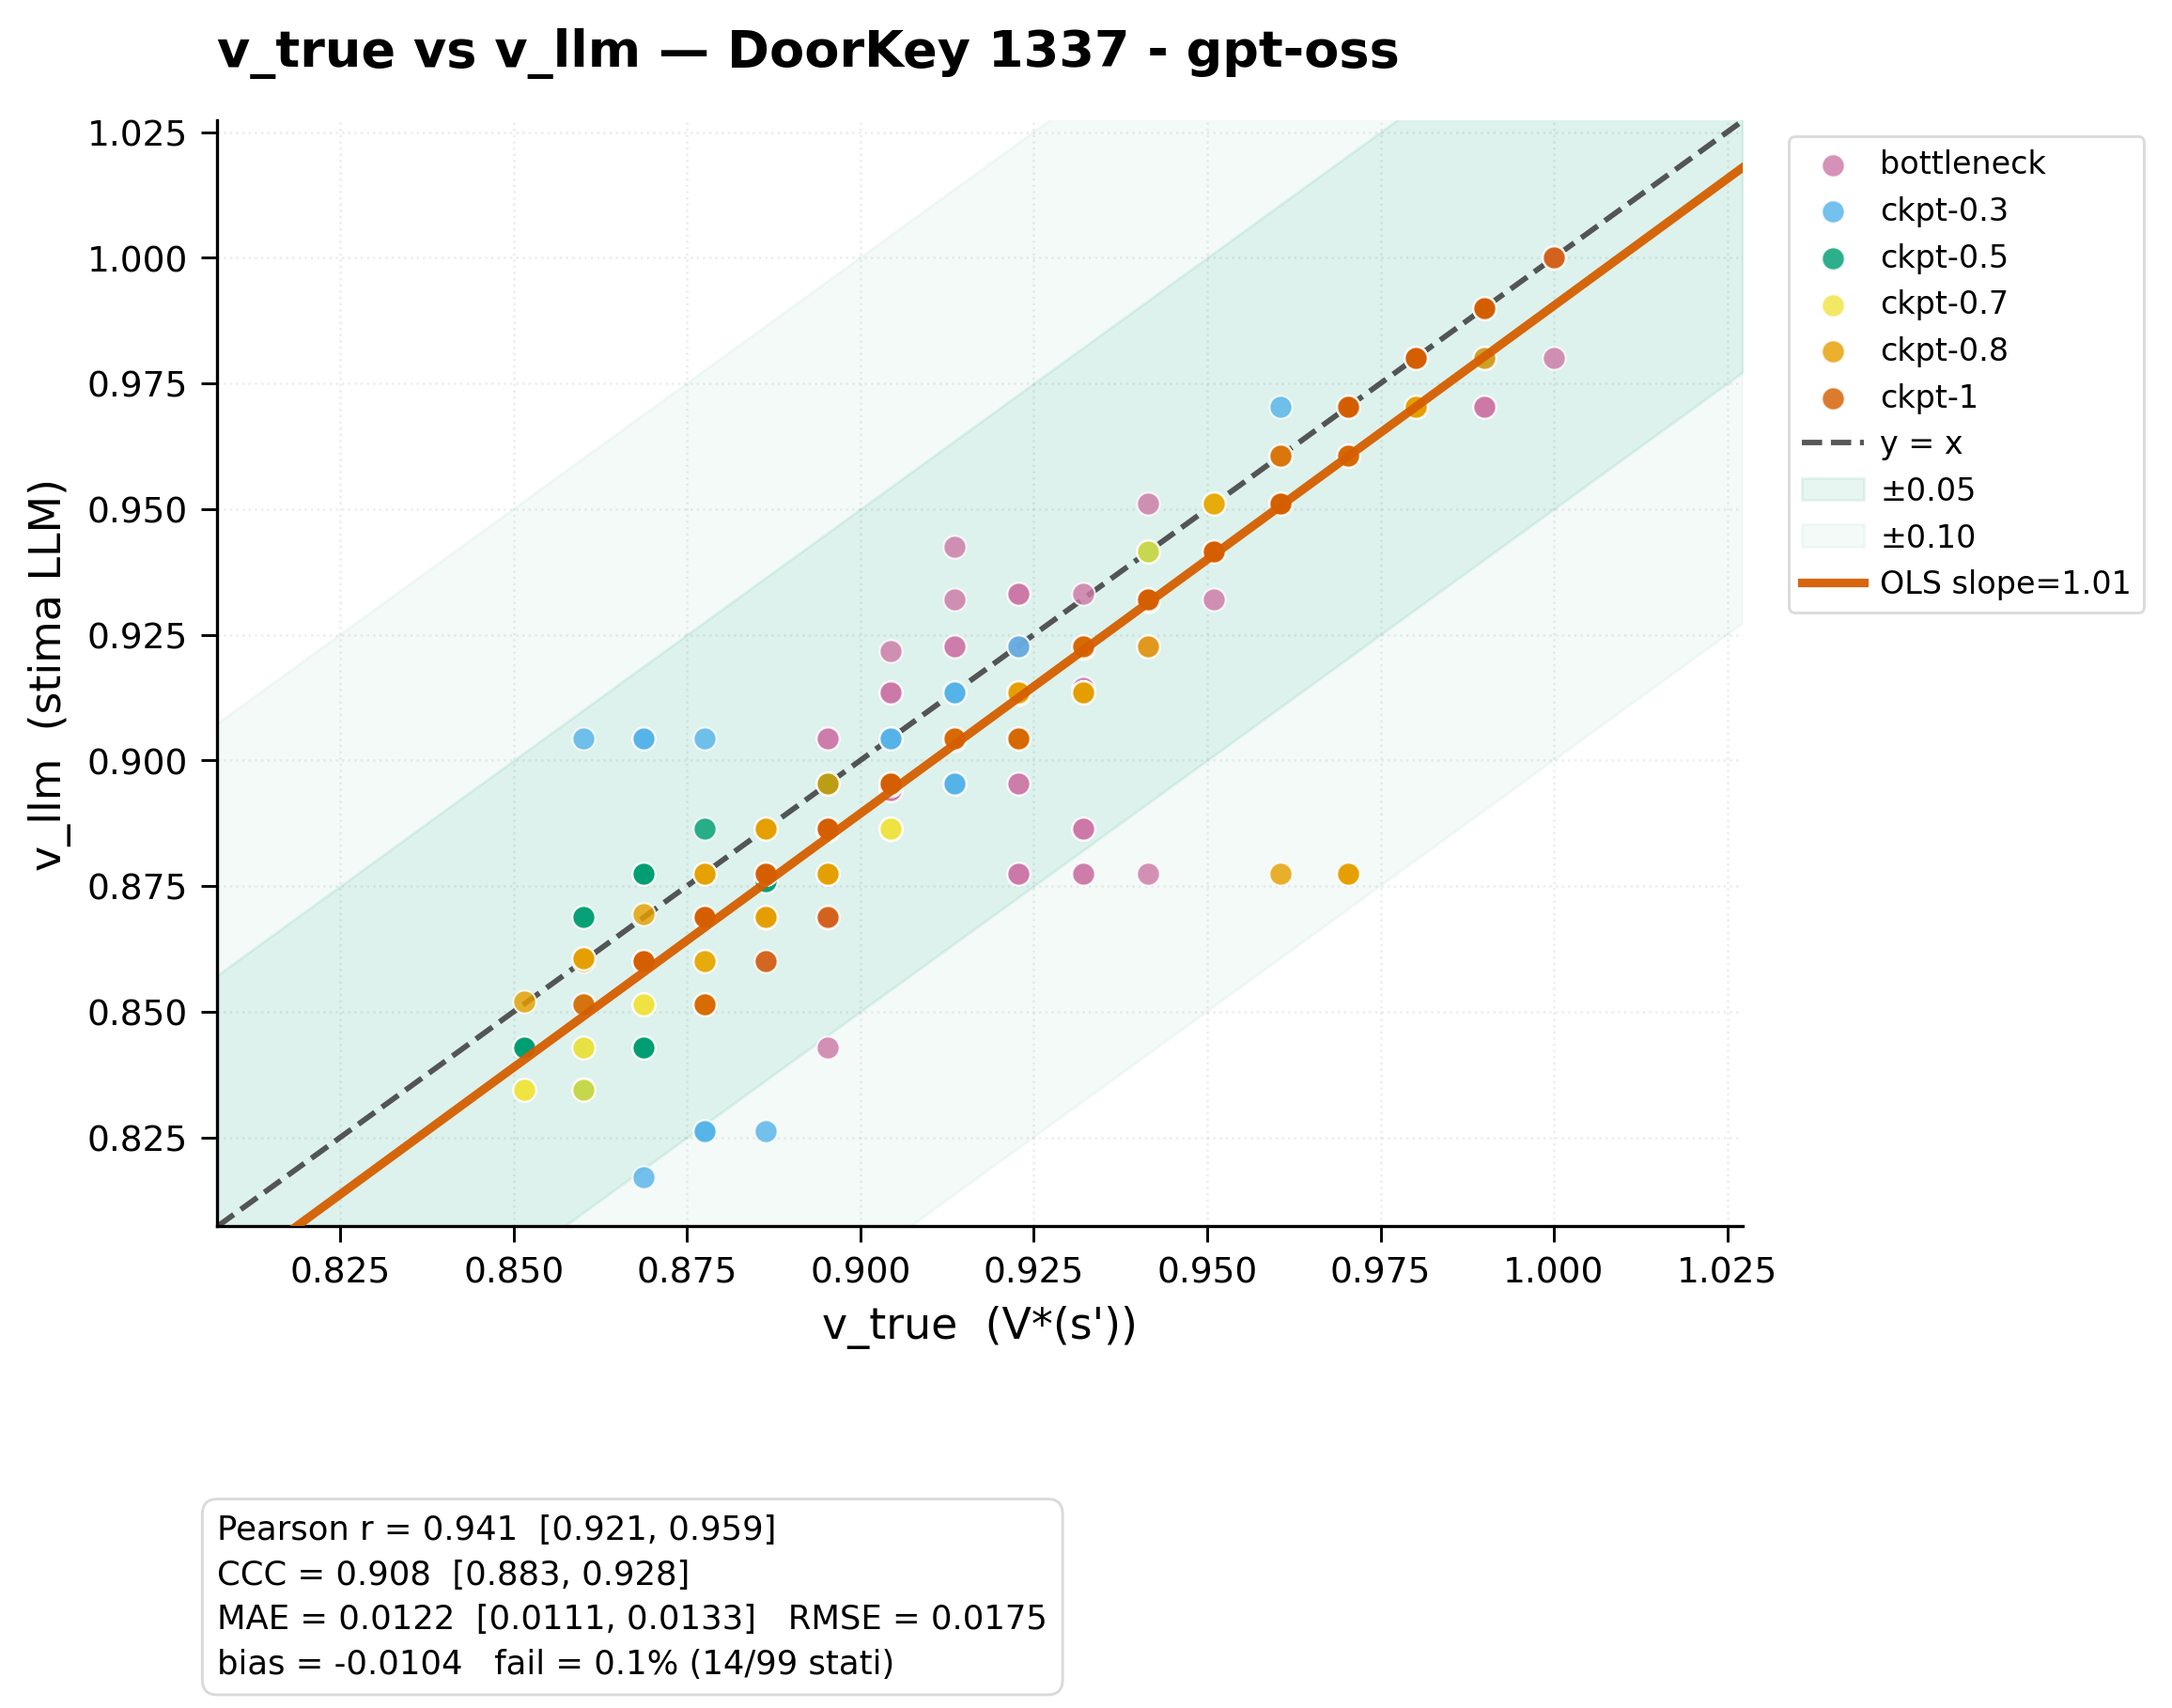
\includegraphics[width=\textwidth]{img/evaluate/grafici/llm_results_doorkey_states_8x8_seed1337_gpt-oss_120b_scatter.png}
\caption{Il pannello confronta $v_{\mathrm{true}}$ sull'asse orizzontale con $v_{\mathrm{llm}}$ sull'asse verticale per lo scenario di base. I punti rappresentano le 85 stime valide; la diagonale $y=x$, le bande $\pm0.05$ e $\pm0.10$ e la retta OLS (pendenza 1.01) sono riportate nel grafico. Il riquadro in basso indica Pearson $r=0.941$, CCC $=0.908$, MAE $=0.0122$, RMSE $=0.0175$, bias $=-0.0104$ e 14 stati falliti su 99, cioè 14/99=14.1\%.}
\label{fig:scatter1337}
\end{figure}

\begin{figure}[H]
\centering
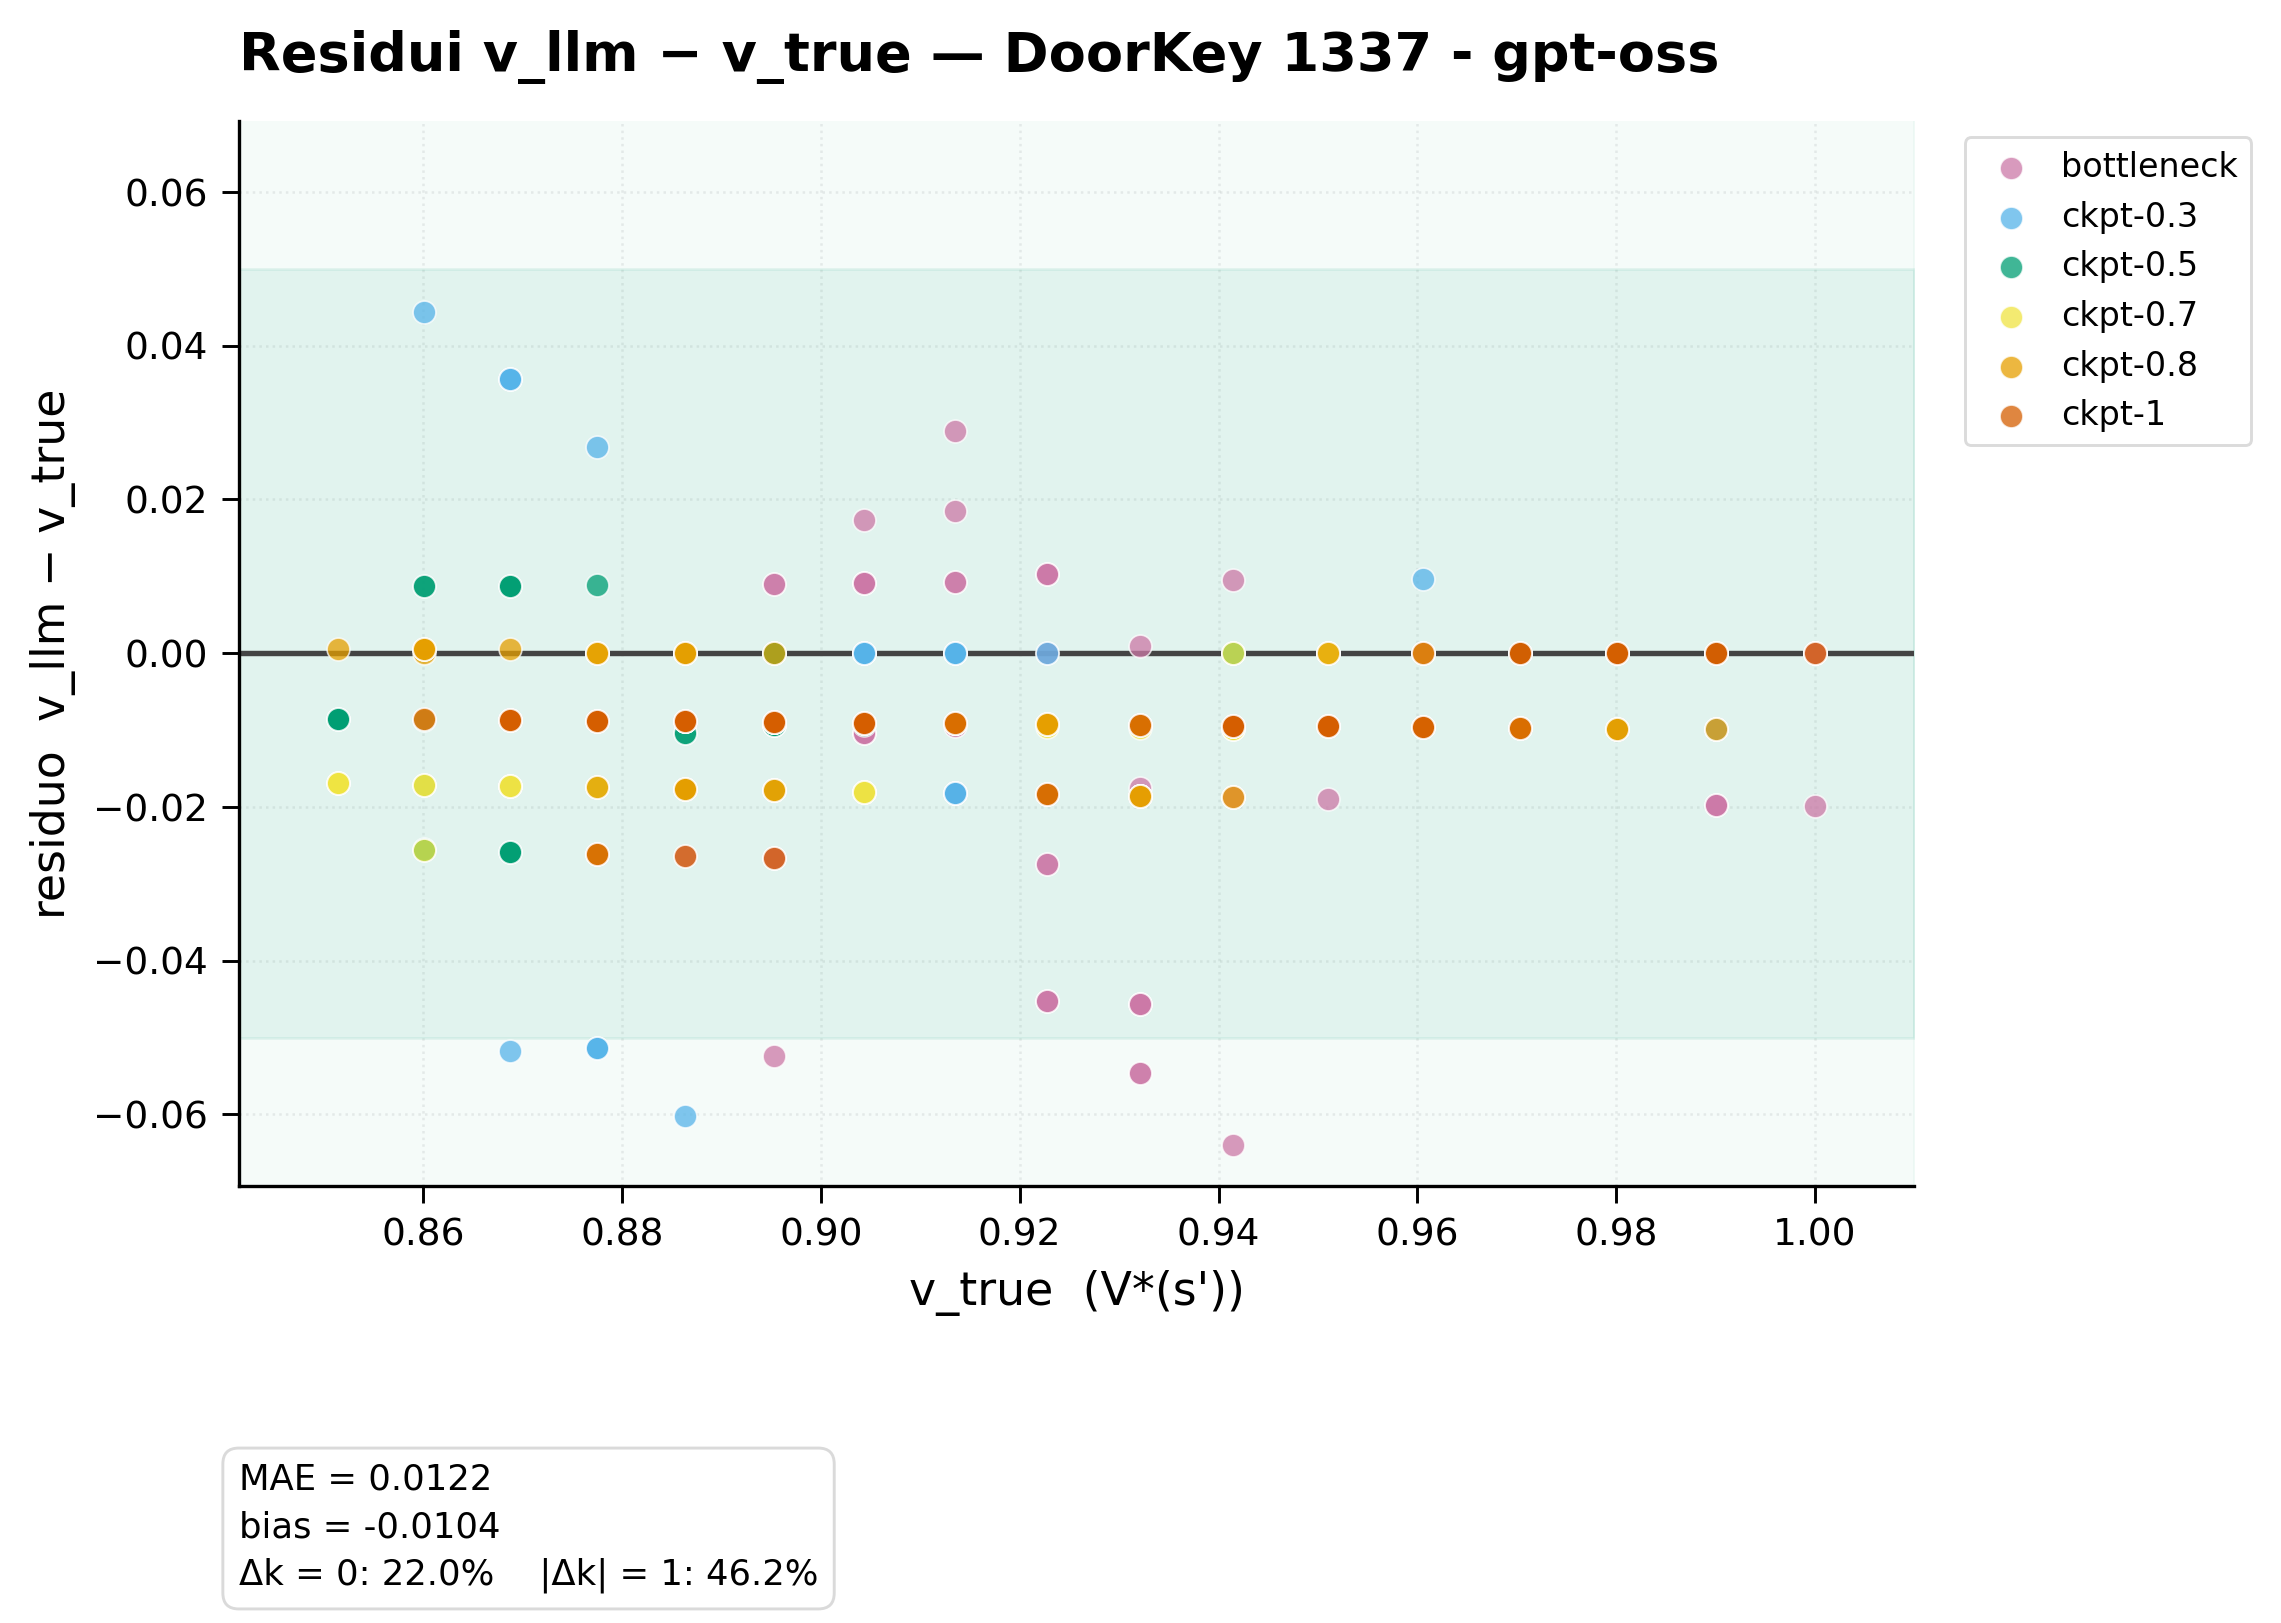
\includegraphics[width=\textwidth]{img/evaluate/grafici/llm_results_doorkey_states_8x8_seed1337_gpt-oss_120b_residuals.png}
\caption{Il pannello mostra il residuo $v_{\mathrm{llm}}-v_{\mathrm{true}}$ per lo scenario di base: l'asse orizzontale riporta il valore di riferimento e quello verticale il residuo. I punti sotto lo zero corrispondono a sottostime. Il riquadro in basso riporta MAE $=0.0122$, bias $=-0.0104$, $\Delta k=0$ nel 22.0\% dei casi e $|\Delta k|=1$ nel 46.2\%. Il bias qui è aggregato sui dati valutati e non è attribuito a un singolo seed.}
\label{fig:resid1337}
\end{figure}

\begin{figure}[H]
\centering
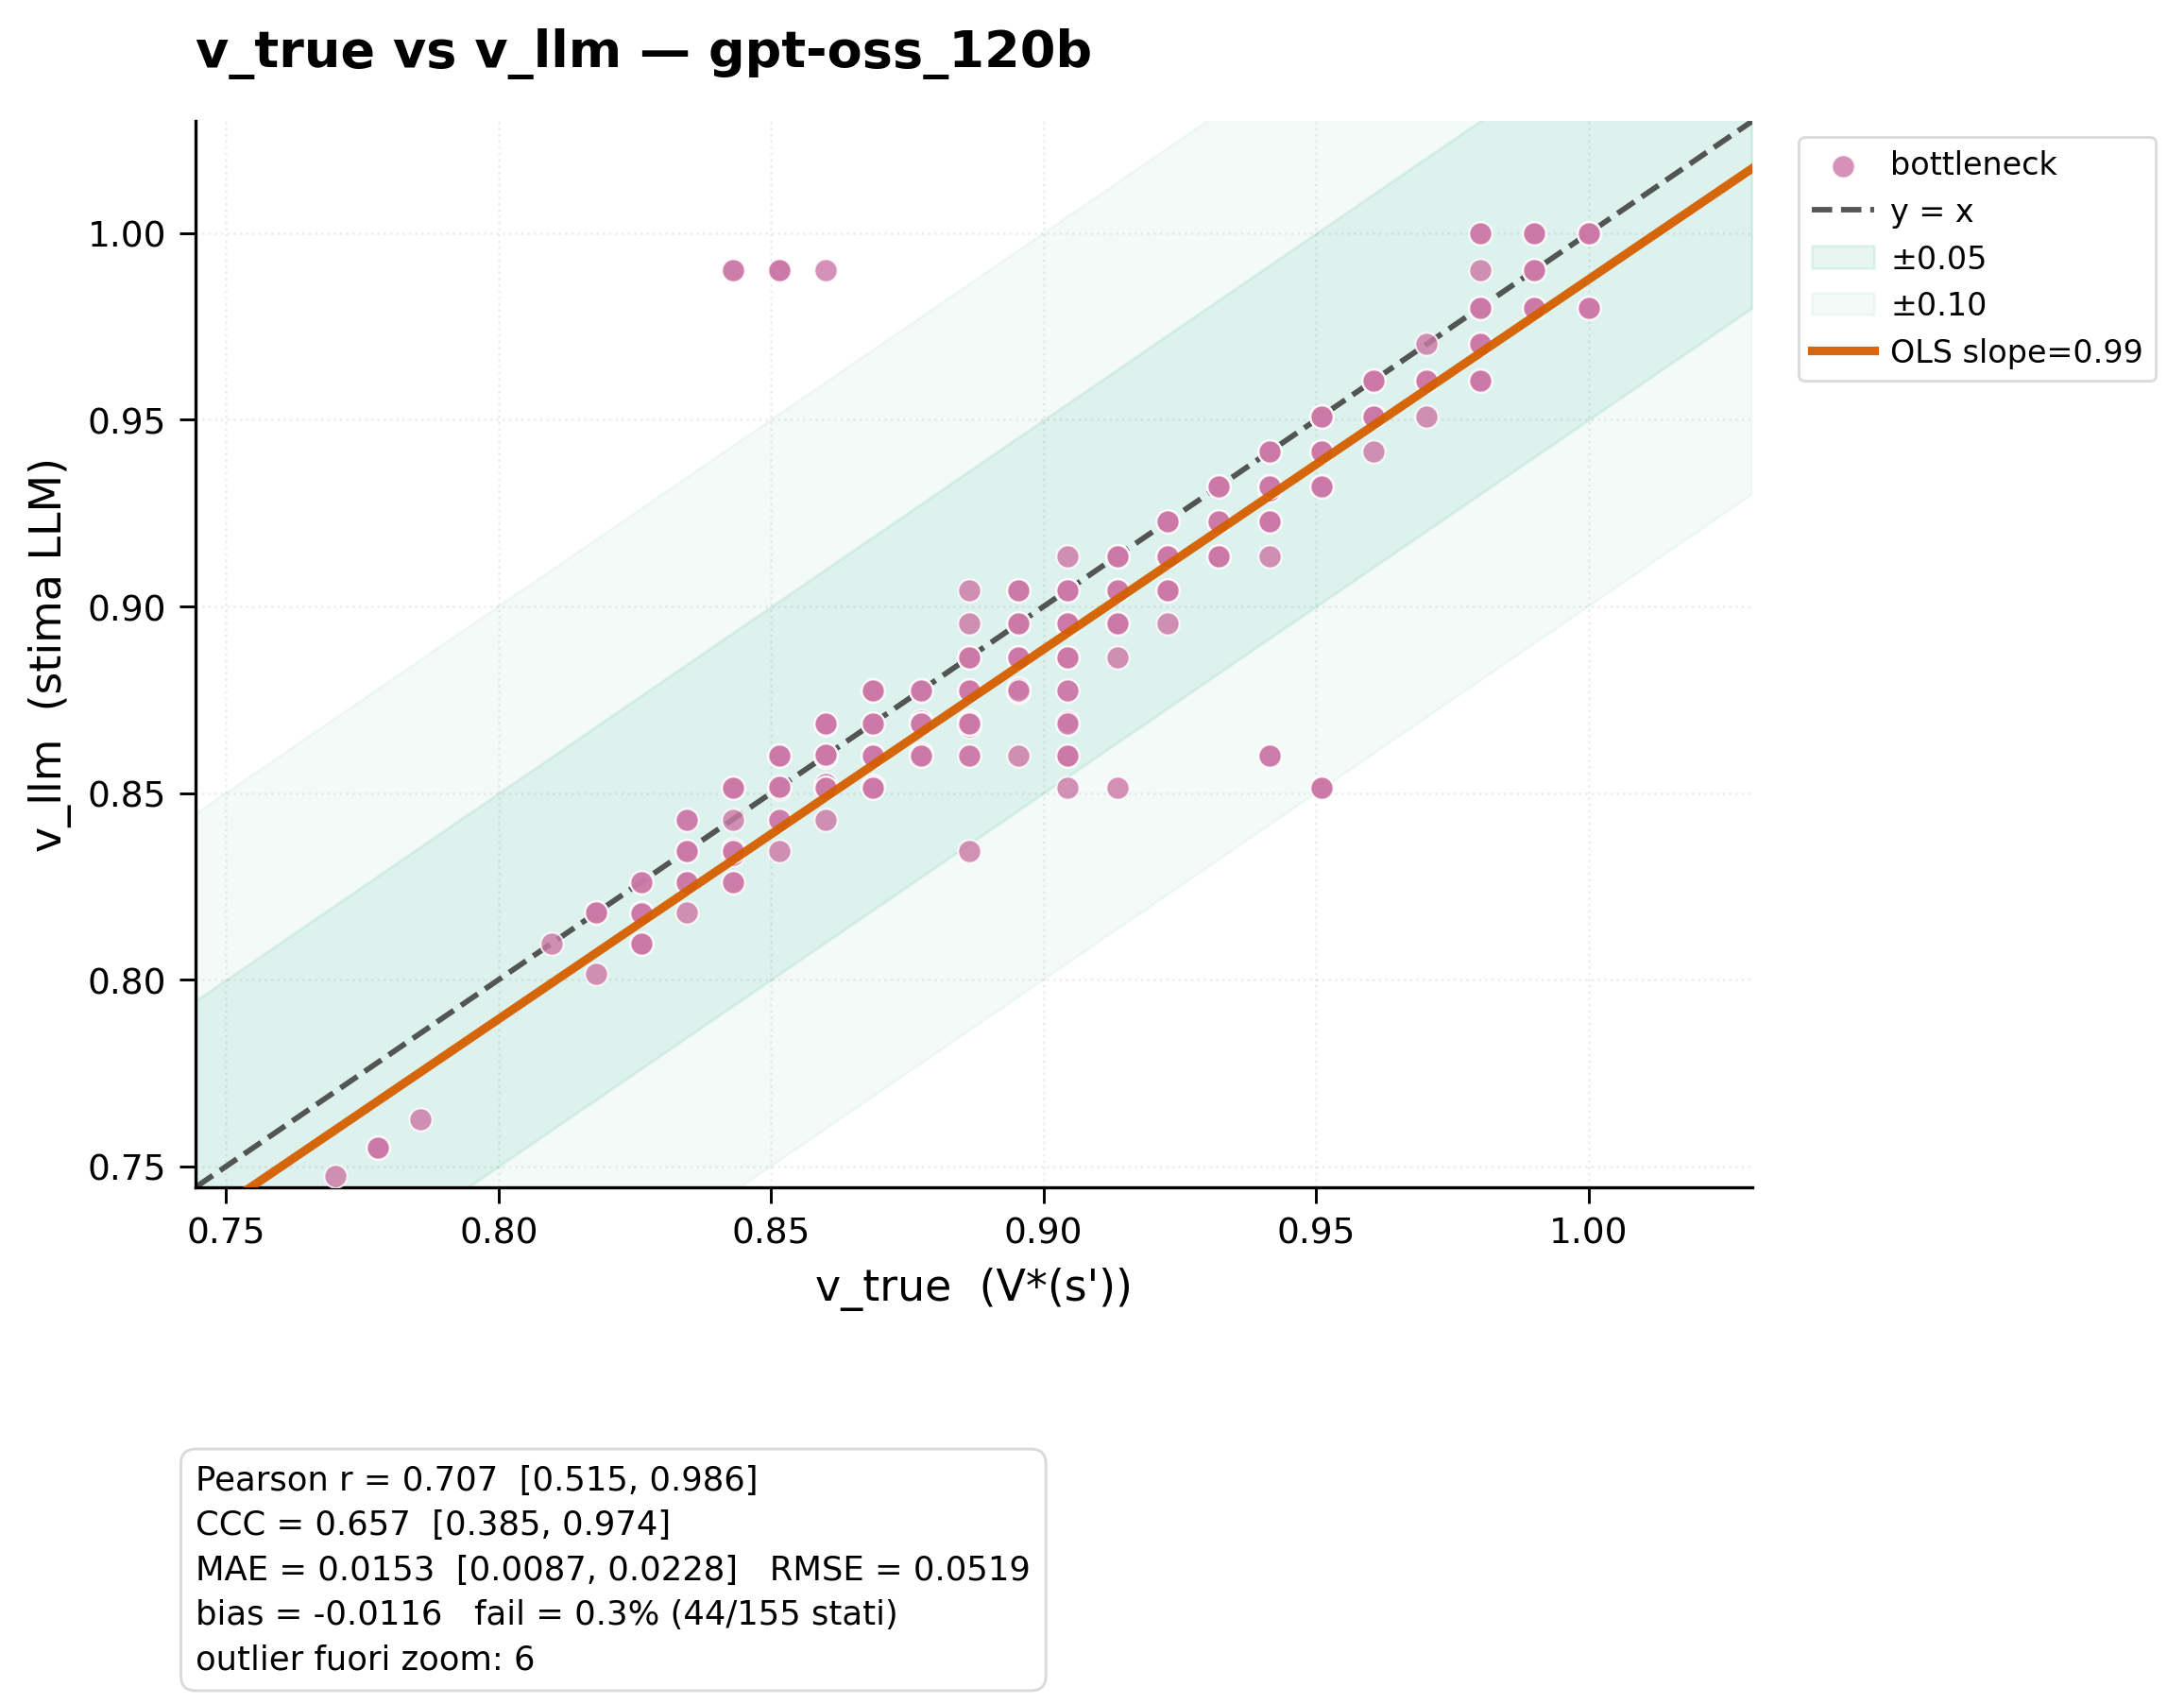
\includegraphics[width=\textwidth]{img/evaluate/grafici/llm_results_doorkey_states_8x8_seeds13507-19920-32455-54937-69693_gpt-oss_120b_scatter.png}
\caption{Il pannello mostra le 111 stime valide dei 155 stati dei cinque layout e confronta $v_{\mathrm{true}}$ con $v_{\mathrm{llm}}$. Tutti i punti appartengono al bucket \texttt{bottleneck}; la diagonale, le bande $\pm0.05$ e $\pm0.10$ e la retta OLS (pendenza 0.99) sono mostrate nel grafico. Il riquadro in basso riporta Pearson $r=0.707$, CCC $=0.657$, MAE $=0.0153$, RMSE $=0.0519$, bias $=-0.0116$, 44 stati falliti su 155 (44/155=28.4\%) e 6 punti fuori dallo zoom. Il grafico non permette di attribuire le differenze a una singola causa.}
\label{fig:scatter5seed}
\end{figure}

\begin{figure}[H]
\centering
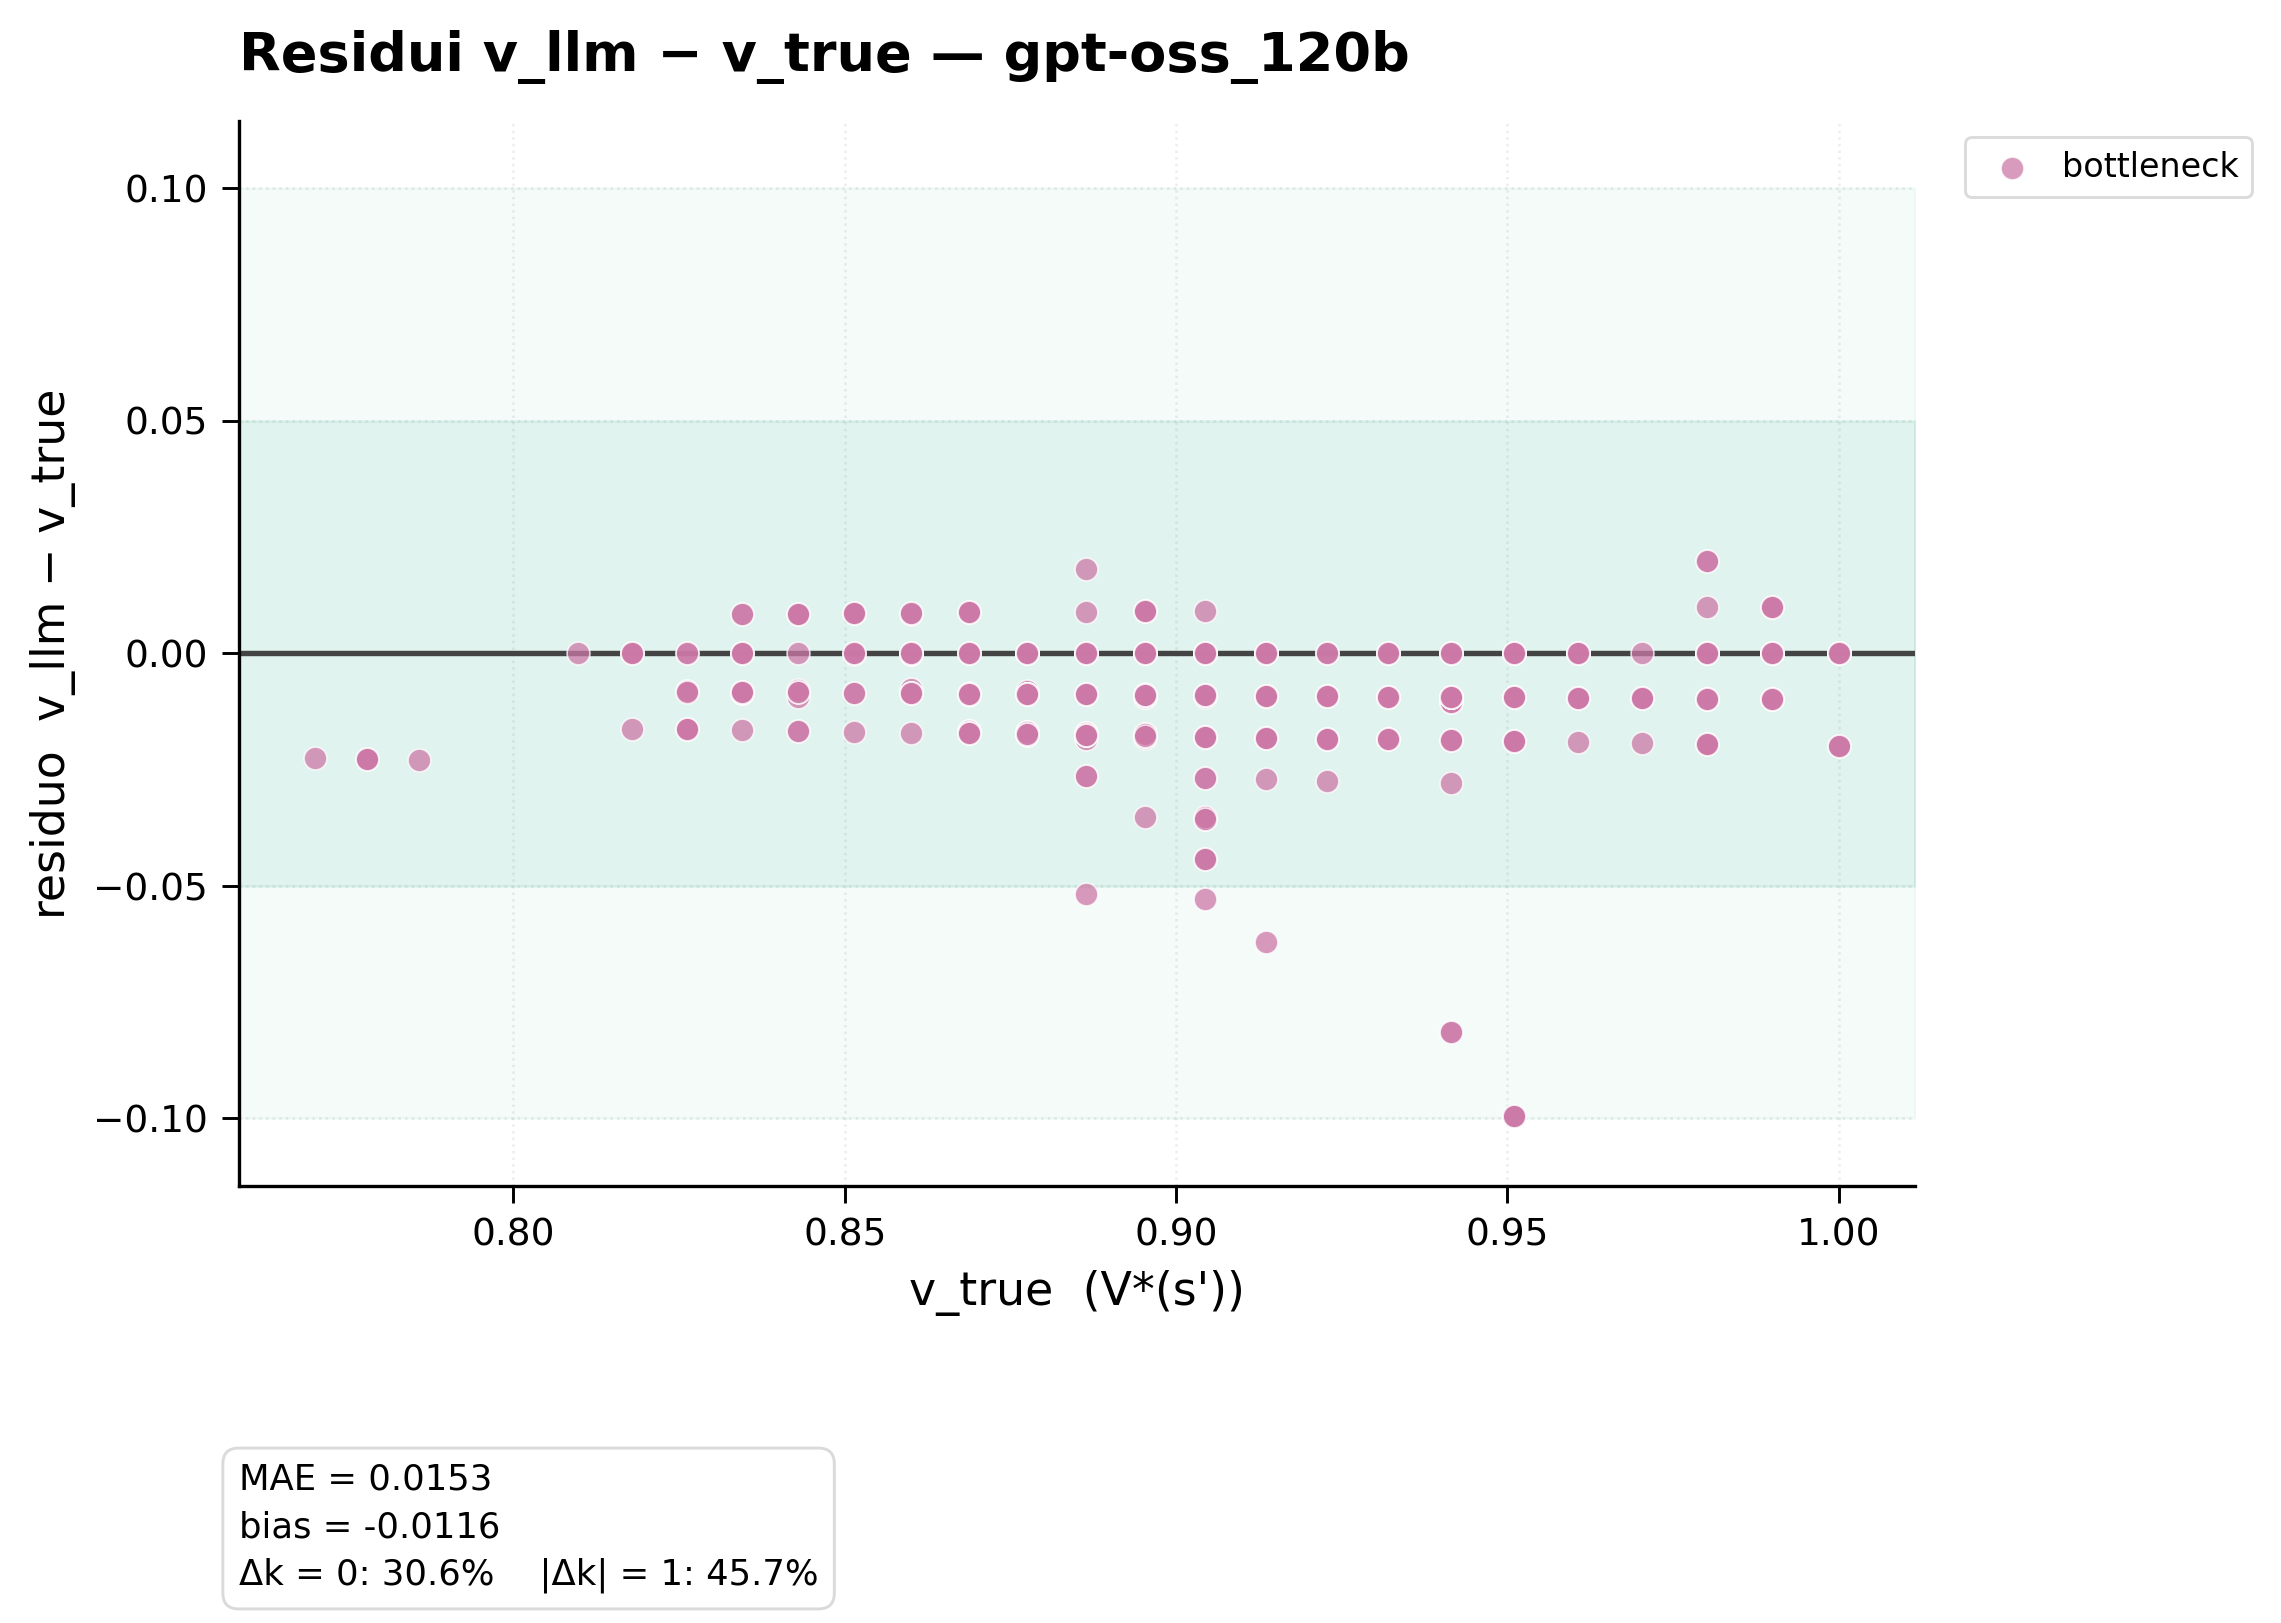
\includegraphics[width=\textwidth]{img/evaluate/grafici/llm_results_doorkey_states_8x8_seeds13507-19920-32455-54937-69693_gpt-oss_120b_residuals.png}
\caption{Il pannello mostra i residui delle 111 stime valide dei 155 stati dei cinque layout: l'asse orizzontale è $v_{\mathrm{true}}$ e quello verticale è $v_{\mathrm{llm}}-v_{\mathrm{true}}$. I punti sotto lo zero indicano sottostime, mentre quelli sopra lo zero indicano sovrastime. Il riquadro in basso riporta MAE $=0.0153$, bias $=-0.0116$, $\Delta k=0$ nel 30.6\% dei casi e $|\Delta k|=1$ nel 45.7\%. Il bias è una statistica aggregata e non dimostra che lo stesso errore si presenti in ciascun seed.}
\label{fig:resid5seed}
\end{figure}

Il bias negativo è calcolato sull'insieme delle osservazioni valide; non descrive un errore da attribuire a ciascun seed. Le Figure \ref{fig:scatter1337} e \ref{fig:scatter5seed} mostrano la dispersione dei punti nei due aggregati.

\section{Qualit\`a dell'azione suggerita}\label{sec:azioni}
L'algoritmo valuta la correttezza dell'azione proposta dal modello. La valutazione tollera piccole imprecisioni numeriche causate dal limite dei decimali.
Dati per lo scenario di base:
\begin{itemize}
\item L'azione suggerita risulta essere la migliore nel 94.1\% dei casi, considerando corrette anche le scelte in pareggio. L'azione casuale ottiene il 16.7\%.
\item Se un pareggio non viene considerato corretto, l'accuratezza Top-1 scende all'84.7\%.
\item Il regret medio delle scelte sub-ottimali ammonta a 0.0011.
\end{itemize}
Le percentuali di selezione dell'azione sono aggregate sugli stati considerati; le Figure \ref{fig:acc1337} e \ref{fig:acc5seed} separano questa metica dal MAE per bucket. Nel campione combinato di cinque layout l'accuratezza Top-1 tie-aware è del 91.9\% e quella strict è dell'82.0\%. I grafici non riportano un'accuratezza azione separata per ogni tipologia di stato.

\begin{figure}[H]
\centering
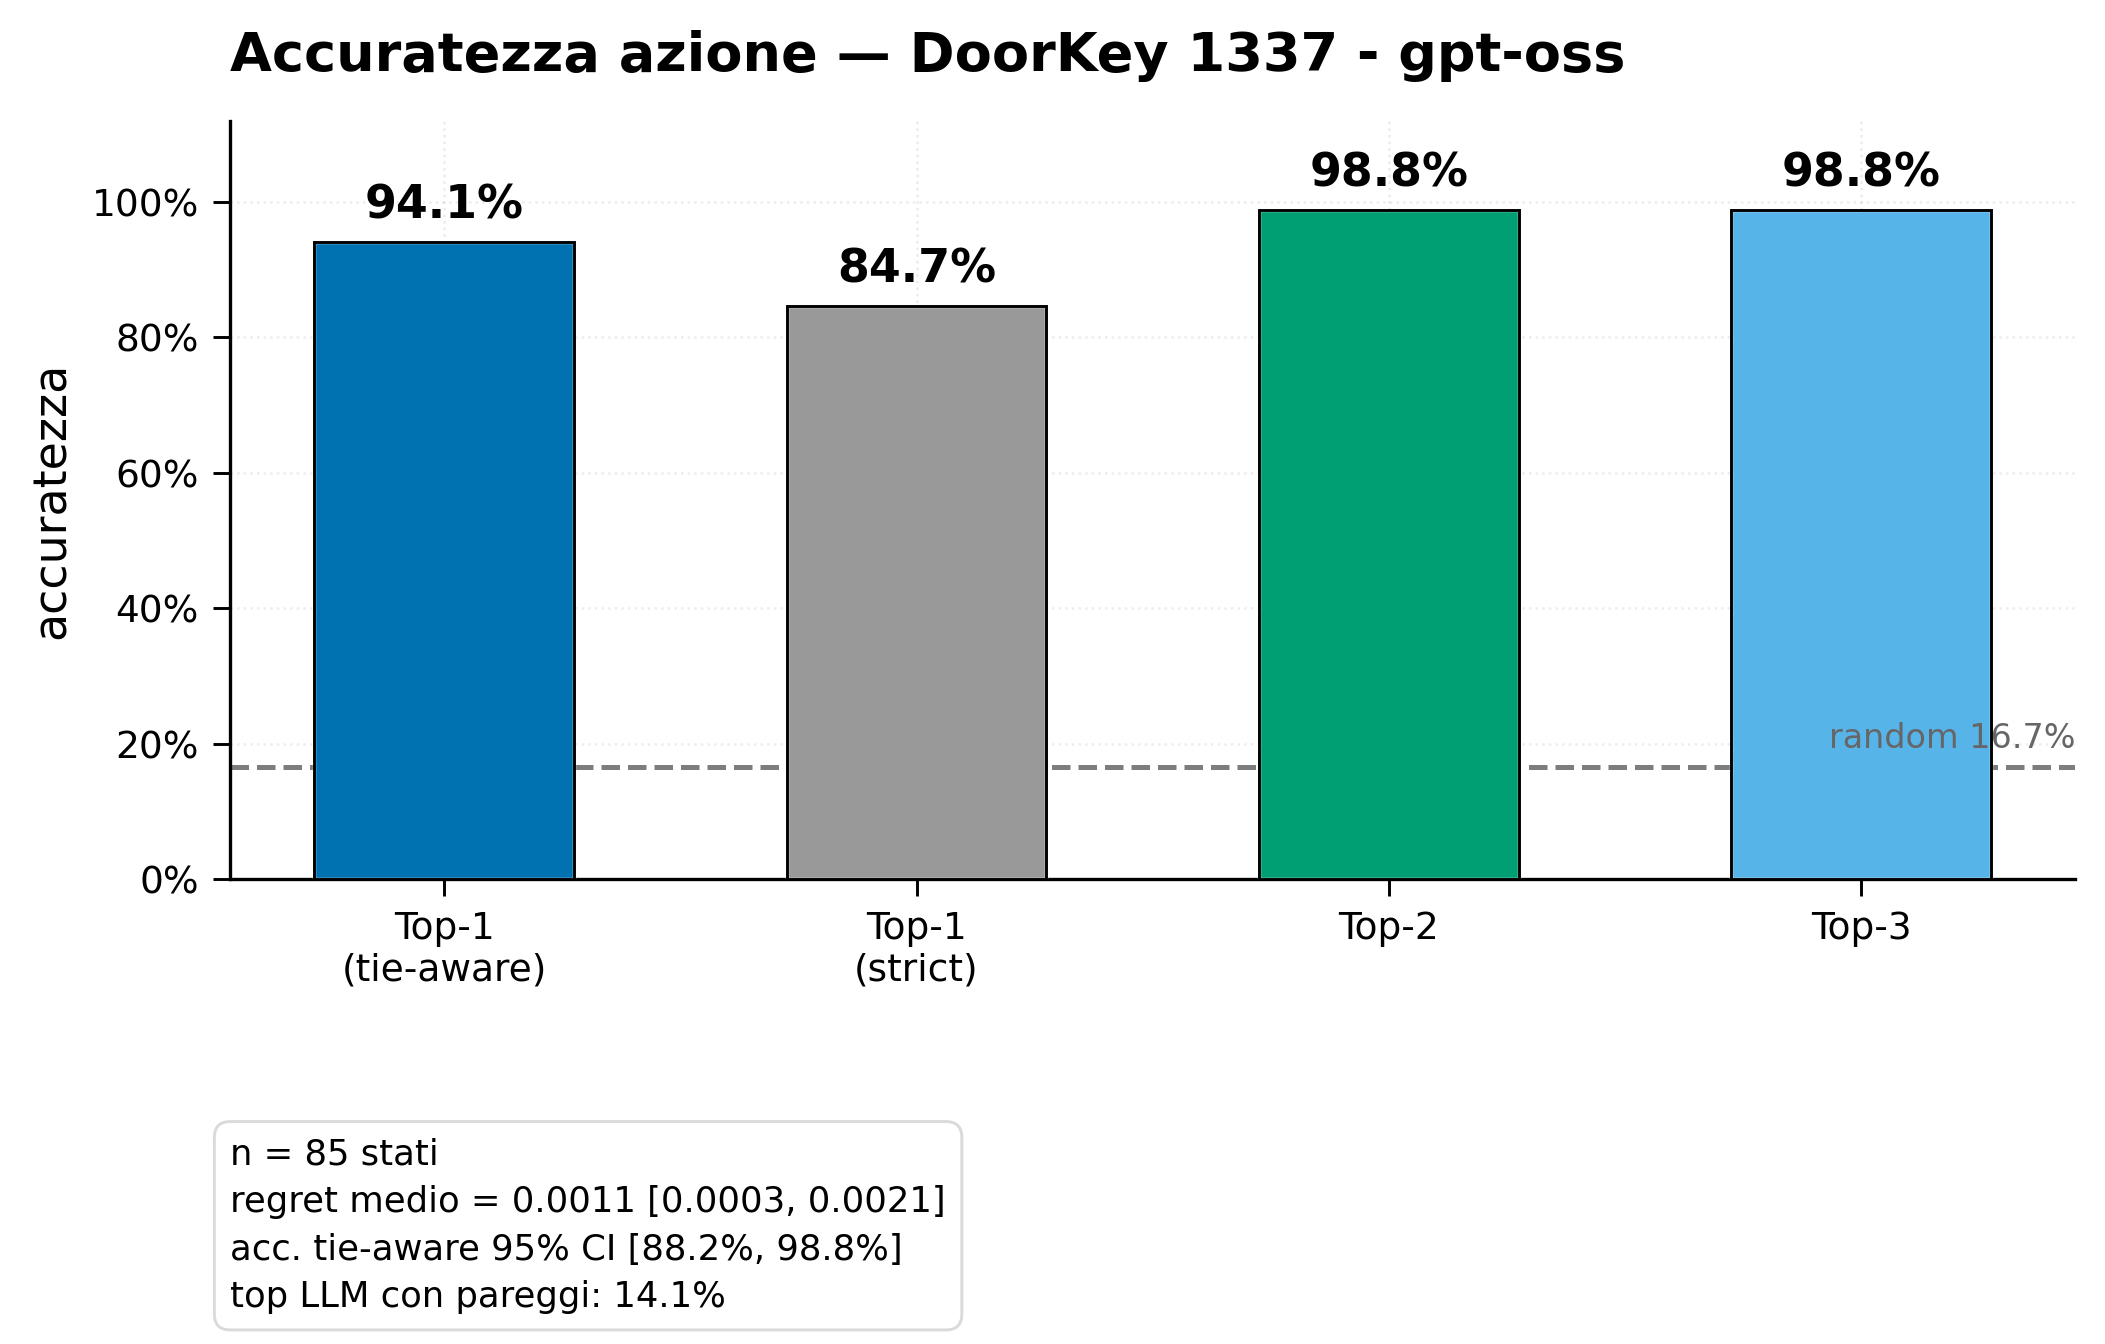
\includegraphics[width=0.48\textwidth]{img/evaluate/grafici/llm_results_doorkey_states_8x8_seed1337_gpt-oss_120b_accuracy.png}
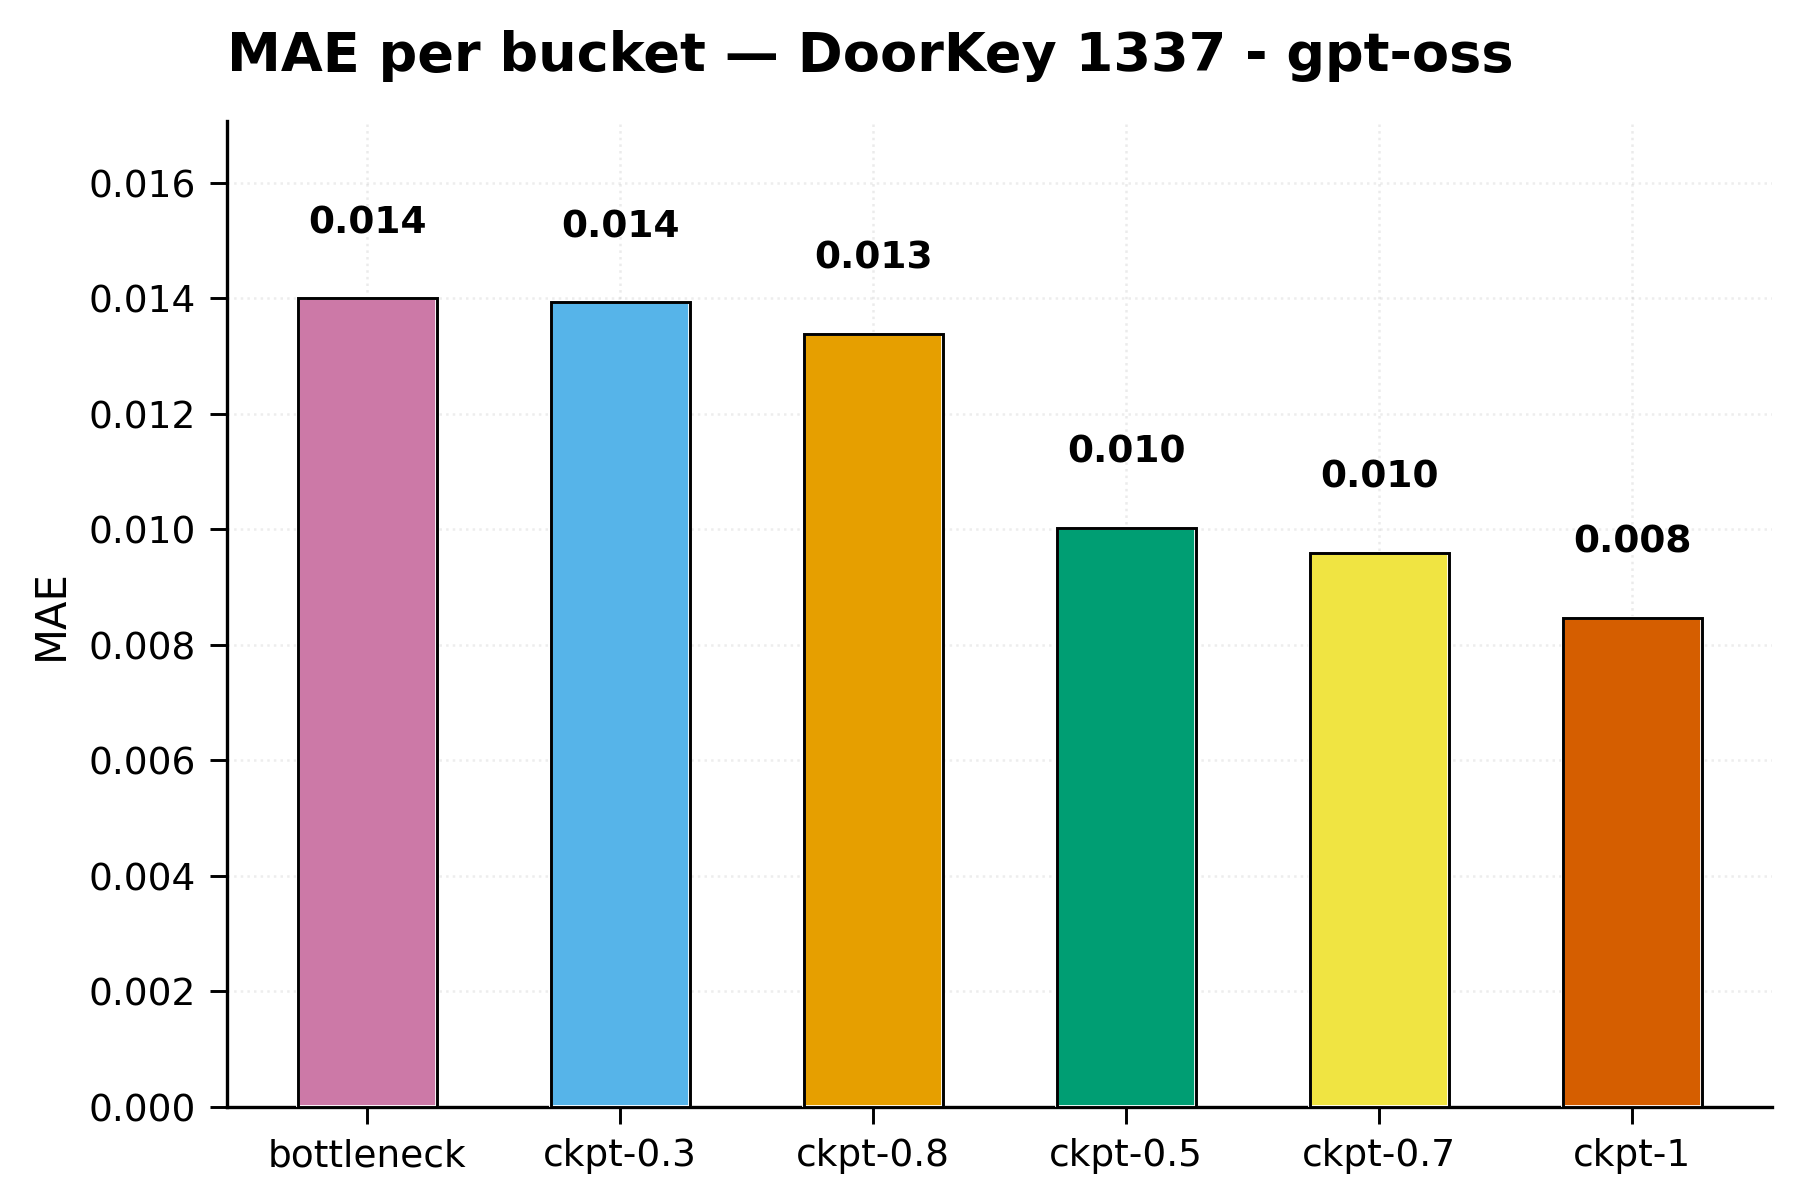
\includegraphics[width=0.48\textwidth]{img/evaluate/grafici/llm_results_doorkey_states_8x8_seed1337_gpt-oss_120b_mae_bucket.png}
\caption{Il pannello sinistro mostra la selezione Top-k aggregata sui 85 stati validi dello scenario di base: Top-1 tie-aware 94.1\%, Top-1 strict 84.7\%, Top-2 98.8\% e Top-3 98.8\%. Il pannello destro è un MAE per bucket, non un grafico Top-k: \texttt{bottleneck} 0.014, \texttt{ckpt-0.3} 0.014, \texttt{ckpt-0.8} 0.013, \texttt{ckpt-0.5} 0.010, \texttt{ckpt-0.7} 0.010 e \texttt{ckpt-1} 0.008. I due pannelli descrivono rispettivamente accuratezza dell'azione ed errore numerico.}
\label{fig:acc1337}
\end{figure}

\begin{figure}[H]
\centering
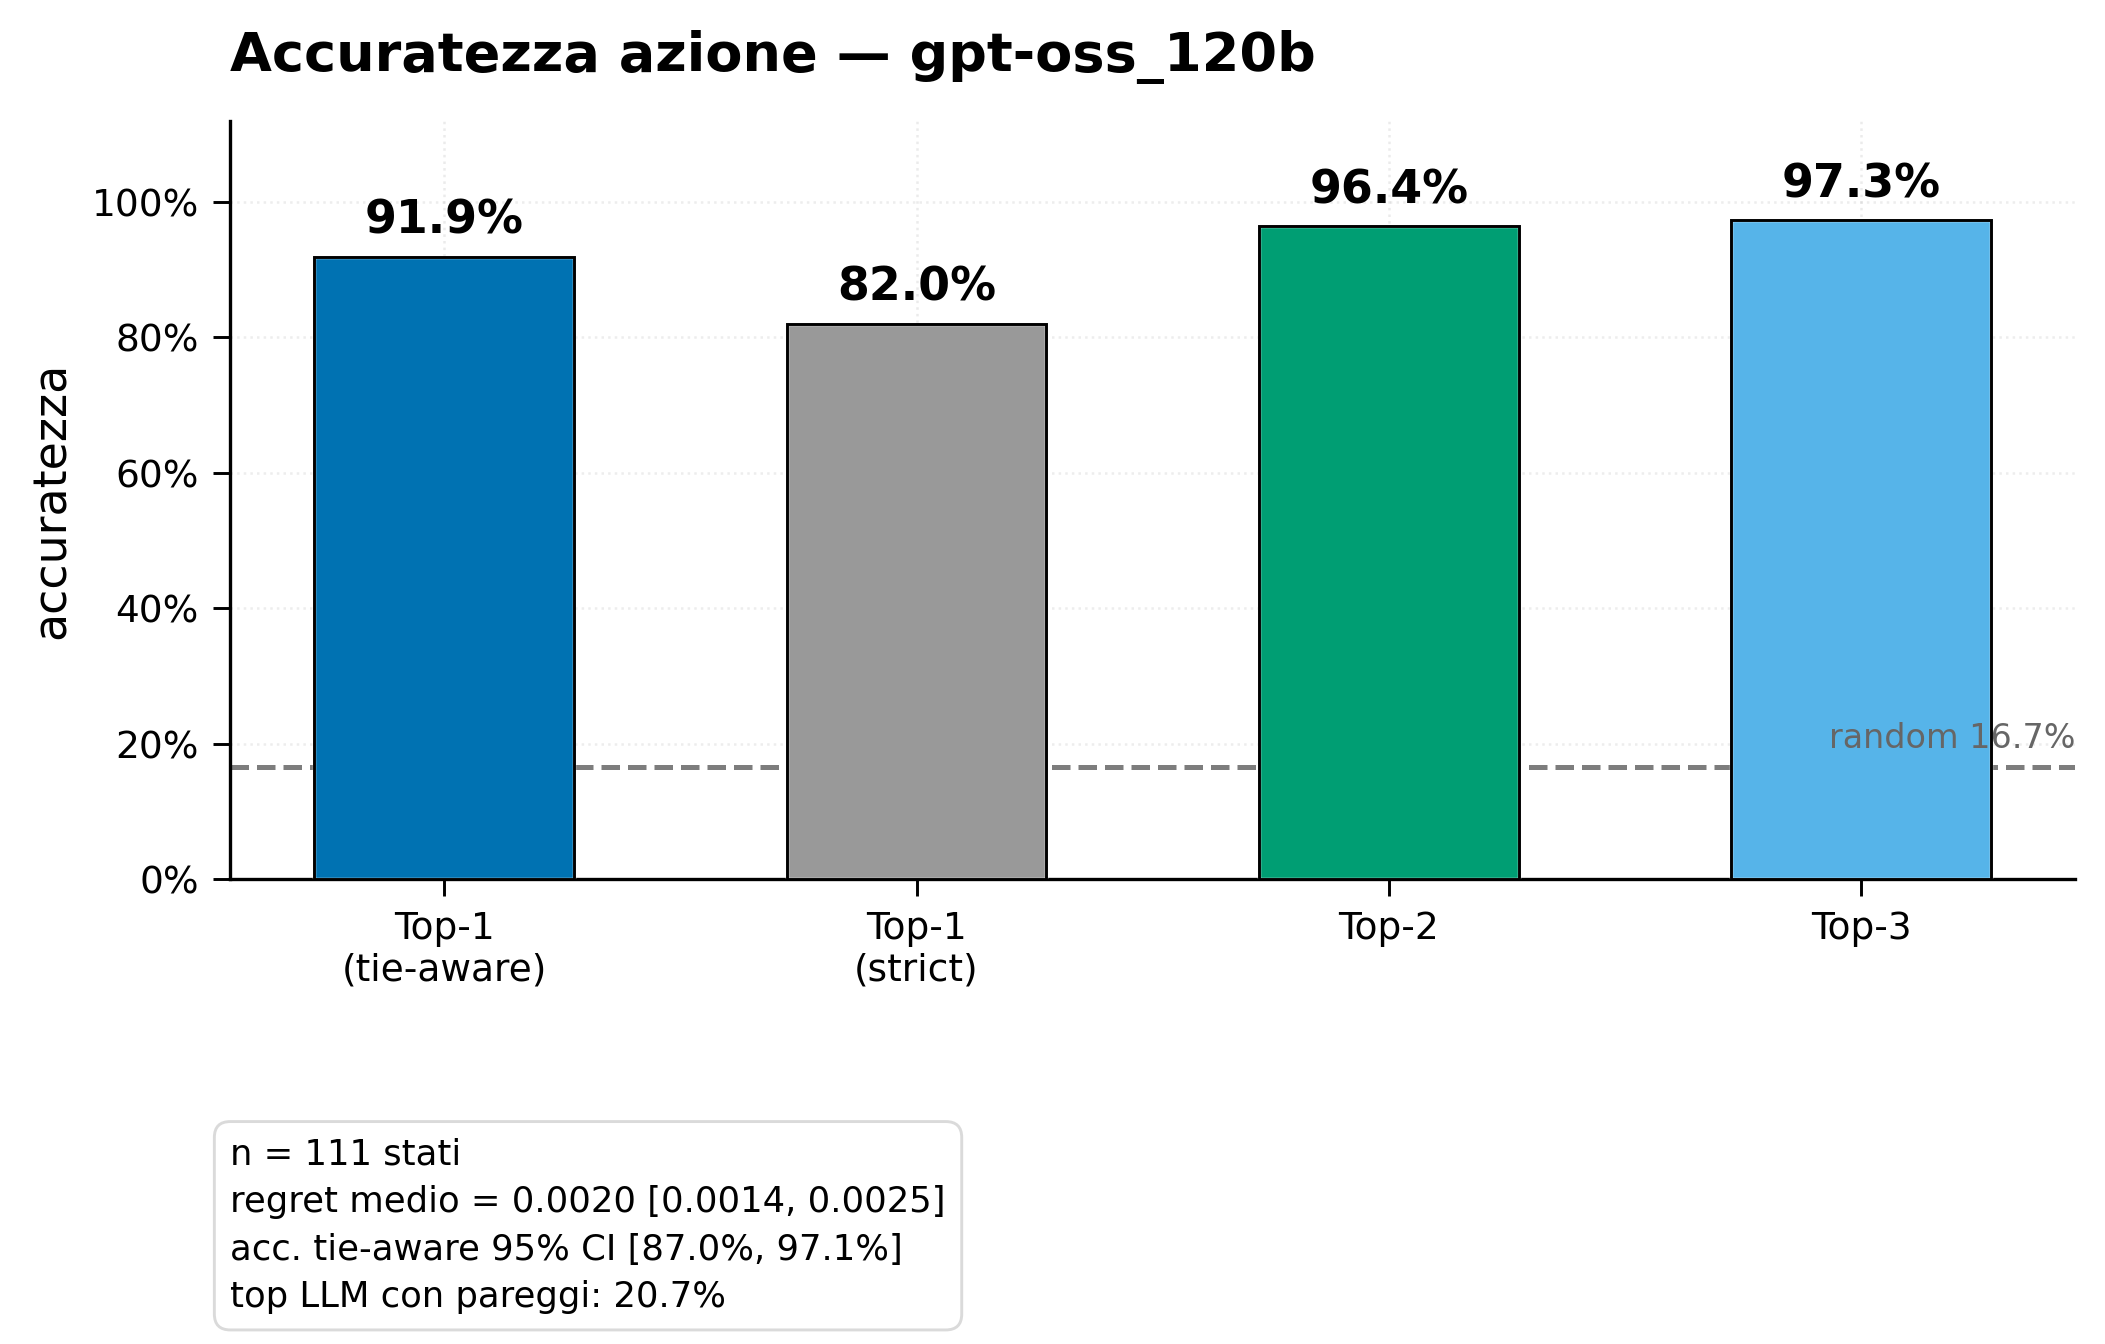
\includegraphics[width=0.48\textwidth]{img/evaluate/grafici/llm_results_doorkey_states_8x8_seeds13507-19920-32455-54937-69693_gpt-oss_120b_accuracy.png}
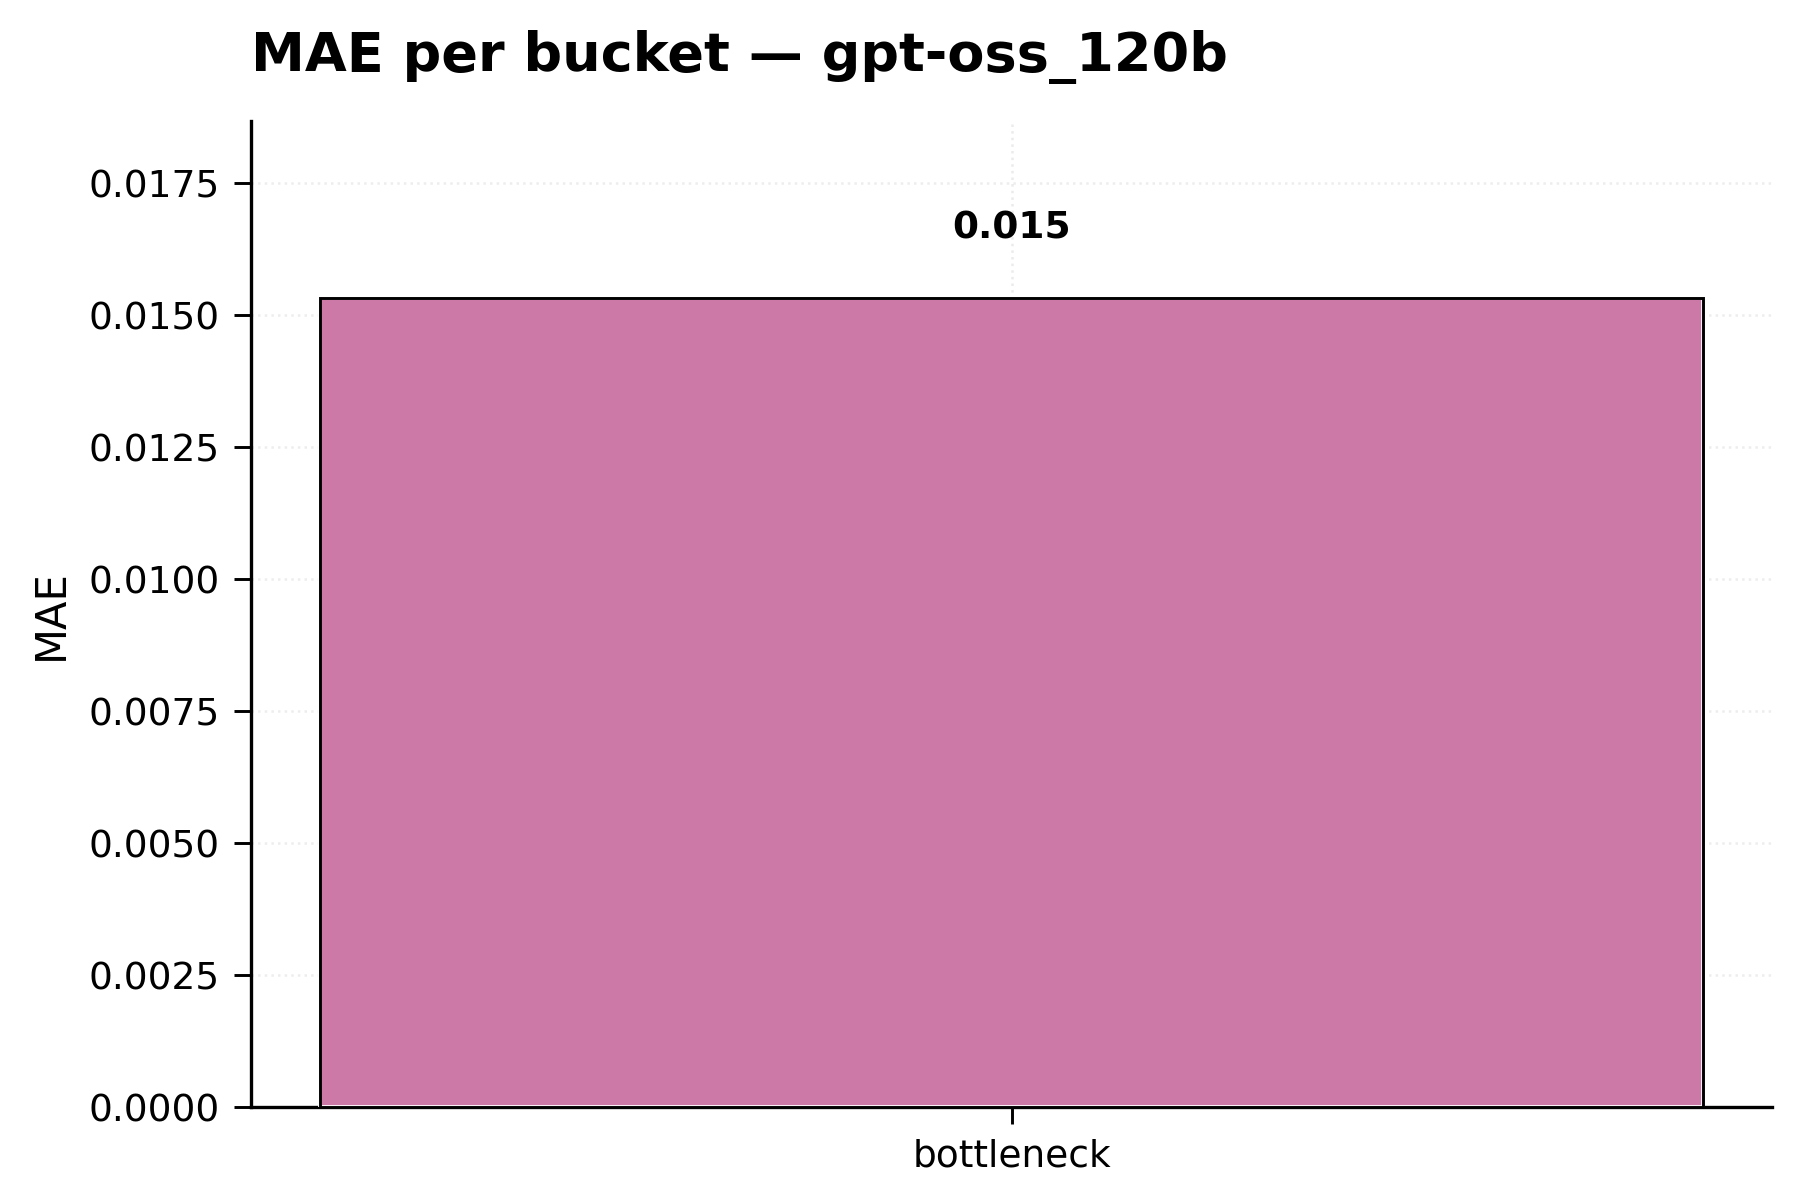
\includegraphics[width=0.48\textwidth]{img/evaluate/grafici/llm_results_doorkey_states_8x8_seeds13507-19920-32455-54937-69693_gpt-oss_120b_mae_bucket.png}
\caption{Il pannello sinistro mostra la selezione Top-k aggregata sui 111 stati validi dei cinque layout: Top-1 tie-aware 91.9\%, Top-1 strict 82.0\%, Top-2 96.4\% e Top-3 97.3\%. Il pannello destro è il MAE per bucket e mostra soltanto \texttt{bottleneck}, con valore 0.015; non presenta una barra per ciascuna tipologia di stato. I valori Top-k e il MAE per bucket non vanno confusi.}
\label{fig:acc5seed}
\end{figure}


\section{Impatto delle stime iniziali}\label{sec:init}
Il codice sorgente per l'agente \`e \path{src/agent/doorkey_qtable_llminit.py}. L'agente usa coordinate relative all'obiettivo intermedio. Le stime calcolate dal modello linguistico vengono inserite inizialmente nella tabella Q; le celle rimanenti partono da zero. Il Q-learning procede quindi su una tabella già parzialmente informata, senza modificare l'obiettivo temporale.

La funzione \path{optimal_policy_metrics} dal file \path{src/agent/doorkey_qtable_llminit.py} confronta le scelte dell'agente con la soluzione calcolata a priori. La prima metrica è l'accordo con la politica ottima, conteggiato con regole che considerano i pareggi. La seconda è la perdita media di valore rispetto a $V^*$. Queste misure vengono calcolate sui nodi incontrati durante le valutazioni.

Il run principale usa 2000 episodi, $\alpha=0.04$, $\gamma=0.99$, decadimento dell'esplorazione 0.99 e 20 coppie stato-azione iniziali. I risultati finali della valutazione greedy su 100 episodi sono:
\begin{itemize}
\item LLM-init: SR=1.00, 13 passi medi, accordo 0.576 e perdita di valore 0.0068.
\item Vanilla (same hp): SR=1.00, 16 passi medi, accordo 0.527 e perdita di valore 0.0075.
\item Vanilla-std, con $\alpha=0.25$ e $\gamma=0.99$: SR=1.00, 16 passi medi, accordo 0.556 e perdita di valore 0.0066.
\end{itemize}
Nel run corrente l'agente LLM-init, con $\alpha=0.04$, raggiunge una curva di successo stabile prima dei due controlli. Il confronto riguarda però una combinazione di inizializzazione e parametri: senza uno sweep riproducibile non è possibile attribuire l'anticipo ad $\alpha$ soltanto, né concludere che un valore basso di $\alpha$ sia sempre migliore. Le Figure \ref{fig:samehp} e \ref{fig:vstd} mostrano i due confronti.

\begin{figure}[H]
\centering

\includegraphics[width=\textwidth]{img/agents/qtable_llminit_seed_1337_gpt-oss_120b_vs_samehp.png}
\caption{Il confronto usa il seed 1337, 2000 episodi, $\alpha=0.04$ e $\gamma=0.95$. Il pannello in alto a sinistra mostra il tasso di successo in addestramento con media mobile su 100 episodi e la valutazione greedy; quello in alto a destra mostra l'errore TD medio per episodio. I pannelli inferiori riportano l'accordo con la politica ottima (0.576 contro 0.527) e la perdita media di valore (0.0068 contro 0.0075). Nella valutazione finale greedy su 100 episodi entrambi gli agenti hanno SR=1.00; le lunghezze medie sono 13 e 16 passi. La figura confronta quindi i risultati finali e l'andamento delle curve, senza isolare l'effetto di una sola variabile.}
\label{fig:samehp}
\end{figure}

\begin{figure}[H]
\centering

\includegraphics[width=\textwidth]{img/agents/qtable_llminit_seed_1337_gpt-oss_120b_vs_std.png}
\caption{Il confronto usa il seed 1337 e 2000 episodi, ma parametri diversi: LLM-init ha $\alpha=0.04$ e $\gamma=0.95$, mentre Vanilla-std ha $\alpha=0.25$ e $\gamma=0.99$. Il pannello in alto a sinistra mostra il tasso di successo in addestramento con media mobile e la valutazione greedy; quello in alto a destra mostra l'errore TD medio per episodio. I pannelli inferiori indicano accordo 0.576 contro 0.556 e perdita di valore 0.0068 contro 0.0066. Entrambe le valutazioni finali greedy su 100 episodi hanno SR=1.00, con 13 e 16 passi medi. La curva del LLM-init sale prima, ma il grafico confronta configurazioni diverse e non dimostra una superiorità universale dell'inizializzazione o di $\alpha$.}
\label{fig:vstd}
\end{figure}

Il secondo ciclo di test usa cinque layout di addestramento, 5000 episodi, $\alpha=0.15$, $\gamma=0.95$ e 400 coppie stato-azione iniziali. I semi addestrati sono 13507, 19920, 32455, 54937 e 69693. I confronti con i controlli seguono la stessa struttura, ma il file e il pannello di valutazione dei confronti riportano il seed 13507, che fa parte dell'addestramento. La Figura \ref{fig:multillminit} distingue la valutazione su quel seed visto dalla valutazione sul seed non visto 69694.

\begin{figure}[H]
\centering

\includegraphics[width=\textwidth]{img/agents/qtable_llminit_multiseed_train13507-19920-32455-54937-69693_evalin13507_evalnew69694_llminit.png}
\caption{Questo pannello riporta i risultati dell'agente LLM-init nel run multi-seed di 5000 episodi con $\alpha=0.15$ e $\gamma=0.95$. Il titolo riporta sia la valutazione sul seed visto 13507 sia quella sul seed non visto 69694; il riquadro in basso fornisce i parametri e i valori del seed visto 13507: SR=1.000, ricompensa media 0.970 e 21 passi medi nella valutazione greedy su 100 episodi. Per il seed non visto 69694 il titolo indica SR=0.000, ricompensa 0.000 e 450 passi. Il pannello superiore destro mostra la curva di addestramento insieme ai riferimenti di valutazione sui due seed; i pannelli inferiori mostrano ricompensa, lunghezza degli episodi ed errore TD.}
\label{fig:multillminit}
\end{figure}

\begin{figure}[H]
\centering

\includegraphics[width=\textwidth]{img/agents/qtable_llminit_multiseed_train13507-19920-32455-54937-69693_evalin13507_evalnew69694_vs_samehp.png}
\caption{Il confronto tra LLM-init e Vanilla (same hp) mostra quattro pannelli del run da 5000 episodi con $\alpha=0.15$ e $\gamma=0.95$. I pannelli superiori riportano il tasso di successo in addestramento con media mobile, la valutazione greedy e l'errore TD; quelli inferiori riportano accordo e perdita di valore. La valutazione riportata è sul seed 13507, che è incluso nell'addestramento, non sul seed non visto 69694. Per LLM-init il riquadro in basso riporta SR=1.000, len=21, agreement=0.671 e loss=0.0038; per il controllo same-hp SR=0.000, len=450, agreement=0.464 e loss=0.0079.}
\label{fig:multisamehp}
\end{figure}

\begin{figure}[H]
\centering

\includegraphics[width=\textwidth]{img/agents/qtable_llminit_multiseed_train13507-19920-32455-54937-69693_evalin13507_evalnew69694_vs_std.png}
\caption{Il confronto tra LLM-init e Vanilla-std mostra gli stessi quattro pannelli del run da 5000 episodi, con LLM-init configurato con $\alpha=0.15$ e il controllo standard con $\alpha=0.15$ e $\gamma=0.99$. Anche in questo caso la valutazione riportata è sul seed 13507, presente nell'addestramento, e non sul seed non visto 69694. I valori finali riportati per LLM-init sono SR=1.000, len=21, agreement=0.671 e loss=0.0038; per Vanilla-std sono SR=0.000, len=450, agreement=0.587 e loss=0.0067. Il grafico non mostra quindi un test di generalizzazione su una mappa non vista.}
\label{fig:multivstd}
\end{figure}

Nel complesso, l'inizializzazione dà un contributo molto netto ai layout addestrati. Sul seed visto 13507 l'agente LLM-init completa il livello con SR=1 e 21 passi, mentre il controllo con gli stessi parametri si ferma a SR=0 e raggiunge il limite di 450 passi. Anche il confronto con il controllo standard mostra lo stesso scarto durante l'addestramento. Sul seed 69694, però, l'agente LLM-init ottiene SR=0 e 450 passi; il controllo standard raggiunge il 17\% sullo stesso seed, un risultato ancora limitato e valutato su una sola mappa. I dati mostrano quindi un forte aiuto sui layout incontrati, ma non risolvono il problema della generalizzazione. Un multi-seed più ampio, con più mappe non viste e repliche indipendenti, potrebbe chiarire quale parte del vantaggio dipenda dall'inizializzazione e quale dalla topologia.


\section{Parametri delle esecuzioni}\label{sec:iperparametri}
I valori riportati di seguito sono le impostazioni dei run effettivamente eseguiti, non una dichiarazione di ottimalità. Nel run principale il tasso di apprendimento è $\alpha=0.04$, il fattore di sconto $\gamma=0.95$, il decadimento dell'esplorazione è 0.99, il limite inferiore di esplorazione è 0.05 e quello dei passi è 450. L'addestramento dura 2000 episodi e la valutazione finale usa 100 episodi greedy. Il controllo standard impiega $\alpha=0.25$ e $\gamma=0.99$.

Il run multi-seed usa $\alpha=0.15$, $\gamma=0.95$, decadimento 0.995, 5000 episodi e 400 coppie stato-azione iniziali. La scelta di questi valori consente di confrontare un run più ampio con quello principale, ma non isola l'effetto di ogni parametro. In particolare, il risultato osservato con $\alpha=0.04$ e LLM-init non dimostra che un valore basso di $\alpha$ sia universalmente migliore; servirebbe uno sweep riproducibile. Il limite di 450 passi interrompe le partite che non raggiungono l'obiettivo entro quel numero di mosse.

\section{Limiti dell'approccio}\label{sec:limiti}
Ogni configurazione è stata eseguita una sola volta. L'esperimento di generalizzazione comprende un solo seed non visto, mentre i cinque layout di addestramento condividono una singola tabella Q: non si tratta di cinque repliche indipendenti dell'intero esperimento. Non è quindi disponibile una stima della varianza. I risultati forniscono evidenze di fattibilità e un punto di partenza concreto, non una prova definitiva dell'efficacia o della generalizzazione.

\section{Conclusione}\label{sec:conclusione}
Il lavoro ha verificato un'ipotesi circoscritta: un insieme ridotto di stime fornite da un modello linguistico può essere inserito nella tabella Q come punto di partenza per il Q-learning. Nel run su seed 1337, l'inizializzazione porta a SR=1 con 13 passi medi e fa salire la curva di successo molto prima del controllo con gli stessi parametri, che alla fine raggiunge anch'esso SR=1 ma con 16 passi. Nel run multi-seed, l'inizializzazione è ancora più netta sul seed visto 13507: l'agente arriva a SR=1 con 21 passi, mentre il controllo con gli stessi parametri non completa il livello nella valutazione finale. Sul singolo seed non visto 69694, però, l'agente ottiene SR=0 e 450 passi.

Il contributo è quindi una forte accelerazione dell'apprendimento sui layout incontrati, accompagnata da percorsi finali più brevi e da una tabella Q leggermente più vicina alla politica ottima. Questi risultati sono promettenti e formano un ottimo punto di partenza, ma non dimostrano la generalizzazione. Una sola esecuzione per configurazione e un solo layout non visto impediscono di stimare la variabilità del metodo; repliche indipendenti e più mappe non viste sono necessarie per separare l'effetto dell'inizializzazione da quello della rappresentazione scelta.

\section{Sviluppi futuri}\label{sec:sviluppi}
I risultati attuali suggeriscono tre direzioni di lavoro.
\begin{enumerate}
\item \textbf{Estensione del set di addestramento.} Più layout e più mappe non viste permetteranno di distinguere la riuscita sui dati addestrati dalla capacità di generalizzare.
\item \textbf{Modelli dedicati.} Un modello addestrato specificamente per stimare valori potrebbe ridurre i tempi necessari a popolare la tabella iniziale.
\item \textbf{Stima in tempo reale.} Il sistema potrebbe interrogare il modello solo quando incontra un nuovo stato, evitando di calcolare in anticipo tutte le coppie stato-azione.
\end{enumerate}
Gli esperimenti attuali restano prove di fattibilità eseguite in tiratura singola.

\clearpage
\appendix
\section{Ambiente FrozenLake}\label{sec:frozenlake}
L'ambiente \path{FrozenLake-v1} introduce esiti probabilistici sulle mosse. Il run FrozenLake slippery usa 18 stati valutati dal modello linguistico e una tabella inizializzata su 40 coppie stato-azione. Sul modello gpt-oss-120b l'errore medio assoluto è 0.1228 e la selezione Top-1 tie-aware è 55.6\%. Nonostante questi valori, la valutazione finale greedy dei tre agenti mostrati raggiunge SR=1.00: LLM-init usa 17 passi medi, contro 23 del controllo same-hp e 22 del controllo standard. Le stime deboli dei valori possono quindi coesistere con un apprendimento riuscito e più rapido; questi dati non indicano un fallimento dell'apprendimento.

\begin{figure}[H]
\centering

\includegraphics[width=\textwidth]{img/evaluate_frozenlake/grafici/frozenlake_llm_8x8_slippery_q_seed1337_gpt-oss_120b_scatter.png}
\caption{Il pannello confronta $v_{\mathrm{true}}$ e $v_{\mathrm{llm}}$ per 72 stime valide su 18 stati dell'ambiente FrozenLake slippery. La diagonale $y=x$, le bande $\pm0.05$ e $\pm0.10$ e la retta OLS (pendenza 1.25) sono mostrate nel grafico. Il riquadro in basso riporta Pearson $r=0.736$, CCC $=0.547$, MAE $=0.1228$, RMSE $=0.1602$, bias $=+0.0923$, 0 stati falliti su 18 e 1 punto fuori dallo zoom. La dispersione descrive l'accuratezza delle stime su questo run, senza spiegarne la causa.}
\label{fig:fl_scatter}
\end{figure}

\begin{figure}[H]
\centering

\includegraphics[width=0.48\textwidth]{img/evaluate_frozenlake/grafici/frozenlake_llm_8x8_slippery_q_seed1337_gpt-oss_120b_accuracy.png}

\includegraphics[width=0.48\textwidth]{img/evaluate_frozenlake/grafici/frozenlake_llm_8x8_slippery_q_seed1337_gpt-oss_120b_mae_bucket.png}
\caption{Il pannello sinistro mostra la selezione Top-k aggregata sui 18 stati: Top-1 tie-aware 55.6\%, Top-1 strict 50.0\%, Top-2 72.2\% e Top-3 83.3\%. Il pannello destro è un MAE per bucket e riporta \texttt{bottleneck} con valore 0.123. Il primo pannello descrive l'accuratezza dell'azione, mentre il secondo descrive l'errore numerico del bucket; non sono due misure per ogni tipologia di stato.}
\label{fig:fl_acc}
\end{figure}

\begin{figure}[H]
\centering

\includegraphics[width=\textwidth]{img/agents/frozenlake_qtable_llminit_8x8_slippery_seed_1337_gpt-oss_120b_vs_samehp.png}
\caption{Il confronto FrozenLake usa il seed 1337, 3000 episodi, $\alpha=0.05$ e $\gamma=0.9$ per LLM-init e gli stessi parametri per il controllo same-hp. Il pannello in alto a sinistra mostra il tasso di successo in addestramento con media mobile e la valutazione greedy; quello in alto a destra mostra l'errore TD medio per episodio. I pannelli inferiori riportano accordo con la politica ottima (0.490 contro 0.453) e perdita media di valore (0.0252 contro 0.0370). Le valutazioni finali greedy su 100 episodi hanno entrambe SR=1.00, ma LLM-init richiede 17 passi medi contro 23 del controllo same-hp.}
\label{fig:fl_samehp}
\end{figure}

\begin{figure}[H]
\centering

\includegraphics[width=\textwidth]{img/agents/frozenlake_qtable_llminit_8x8_slippery_seed_1337_gpt-oss_120b_vs_std.png}
\caption{Il confronto FrozenLake usa il seed 1337 e 3000 episodi, con LLM-init ad $\alpha=0.05$ e $\gamma=0.9$ e Vanilla-std ad $\alpha=0.1$ e $\gamma=0.99$. I pannelli mostrano lo stesso andamento di addestramento, errore TD, accordo con la politica ottima e perdita media di valore. I pannelli inferiori indicano accordo 0.490 contro 0.472 e perdita 0.0252 contro 0.0338. Entrambe le valutazioni finali greedy su 100 episodi hanno SR=1.00, con 17 e 22 passi medi. Non si tratta quindi di un fallimento dell'apprendimento, ma di un confronto fra due configurazioni con parametri diversi.}
\label{fig:fl_vstd}
\end{figure}

\clearpage
\begin{thebibliography}{9}
\bibitem{sutton2018} Sutton, R. S., Barto, A. G. \textit{Reinforcement Learning: An Introduction}, 2nd ed., MIT Press, 2018.
\bibitem{minigrid2023} Chevalier-Boisvert, M. et al. MiniGrid and MiniWorld. \textit{NeurIPS} 36, 2023.
\end{thebibliography}

\end{document}
